\chapterOrPart{Literature Review}\label{ch:literature}

\begin{explanation}
    It is common practice to have a literature review in a thesis where the state-of-the-art and the relevant literature are discussed. But it must not necessarily be done in a separate chapter. It can also be a section in another chapter.

    In the appendix about useful packages, you will find more info about \texttt{biblatex}, a package used for managing and formatting citations and bibliographies. Please also consult the guidelines for using other people's work, in the appendix on formatting.
    
    Feel free to alter the name of the chapter and/or the sections.
\end{explanation}


%%%%%%%% VERSION 2 %%%%%%%%
\section{Energy}
Energy is a conserved physical quantity that denotes a system's capacity to carry out operations or bring about physical change.
It is a fundamental requirement for modern societies that underpins essential services such as electricity generation, transportation, heating, industrial production, and digital infrastructure. In recent decades, energy has become an increasingly prominent topic in both academic and policy discussions. This is driven not only by the ongoing energy transition toward low-carbon systems, but also by the persistent growth in global energy demand.

\begin{figure}[ht]
    \centering
    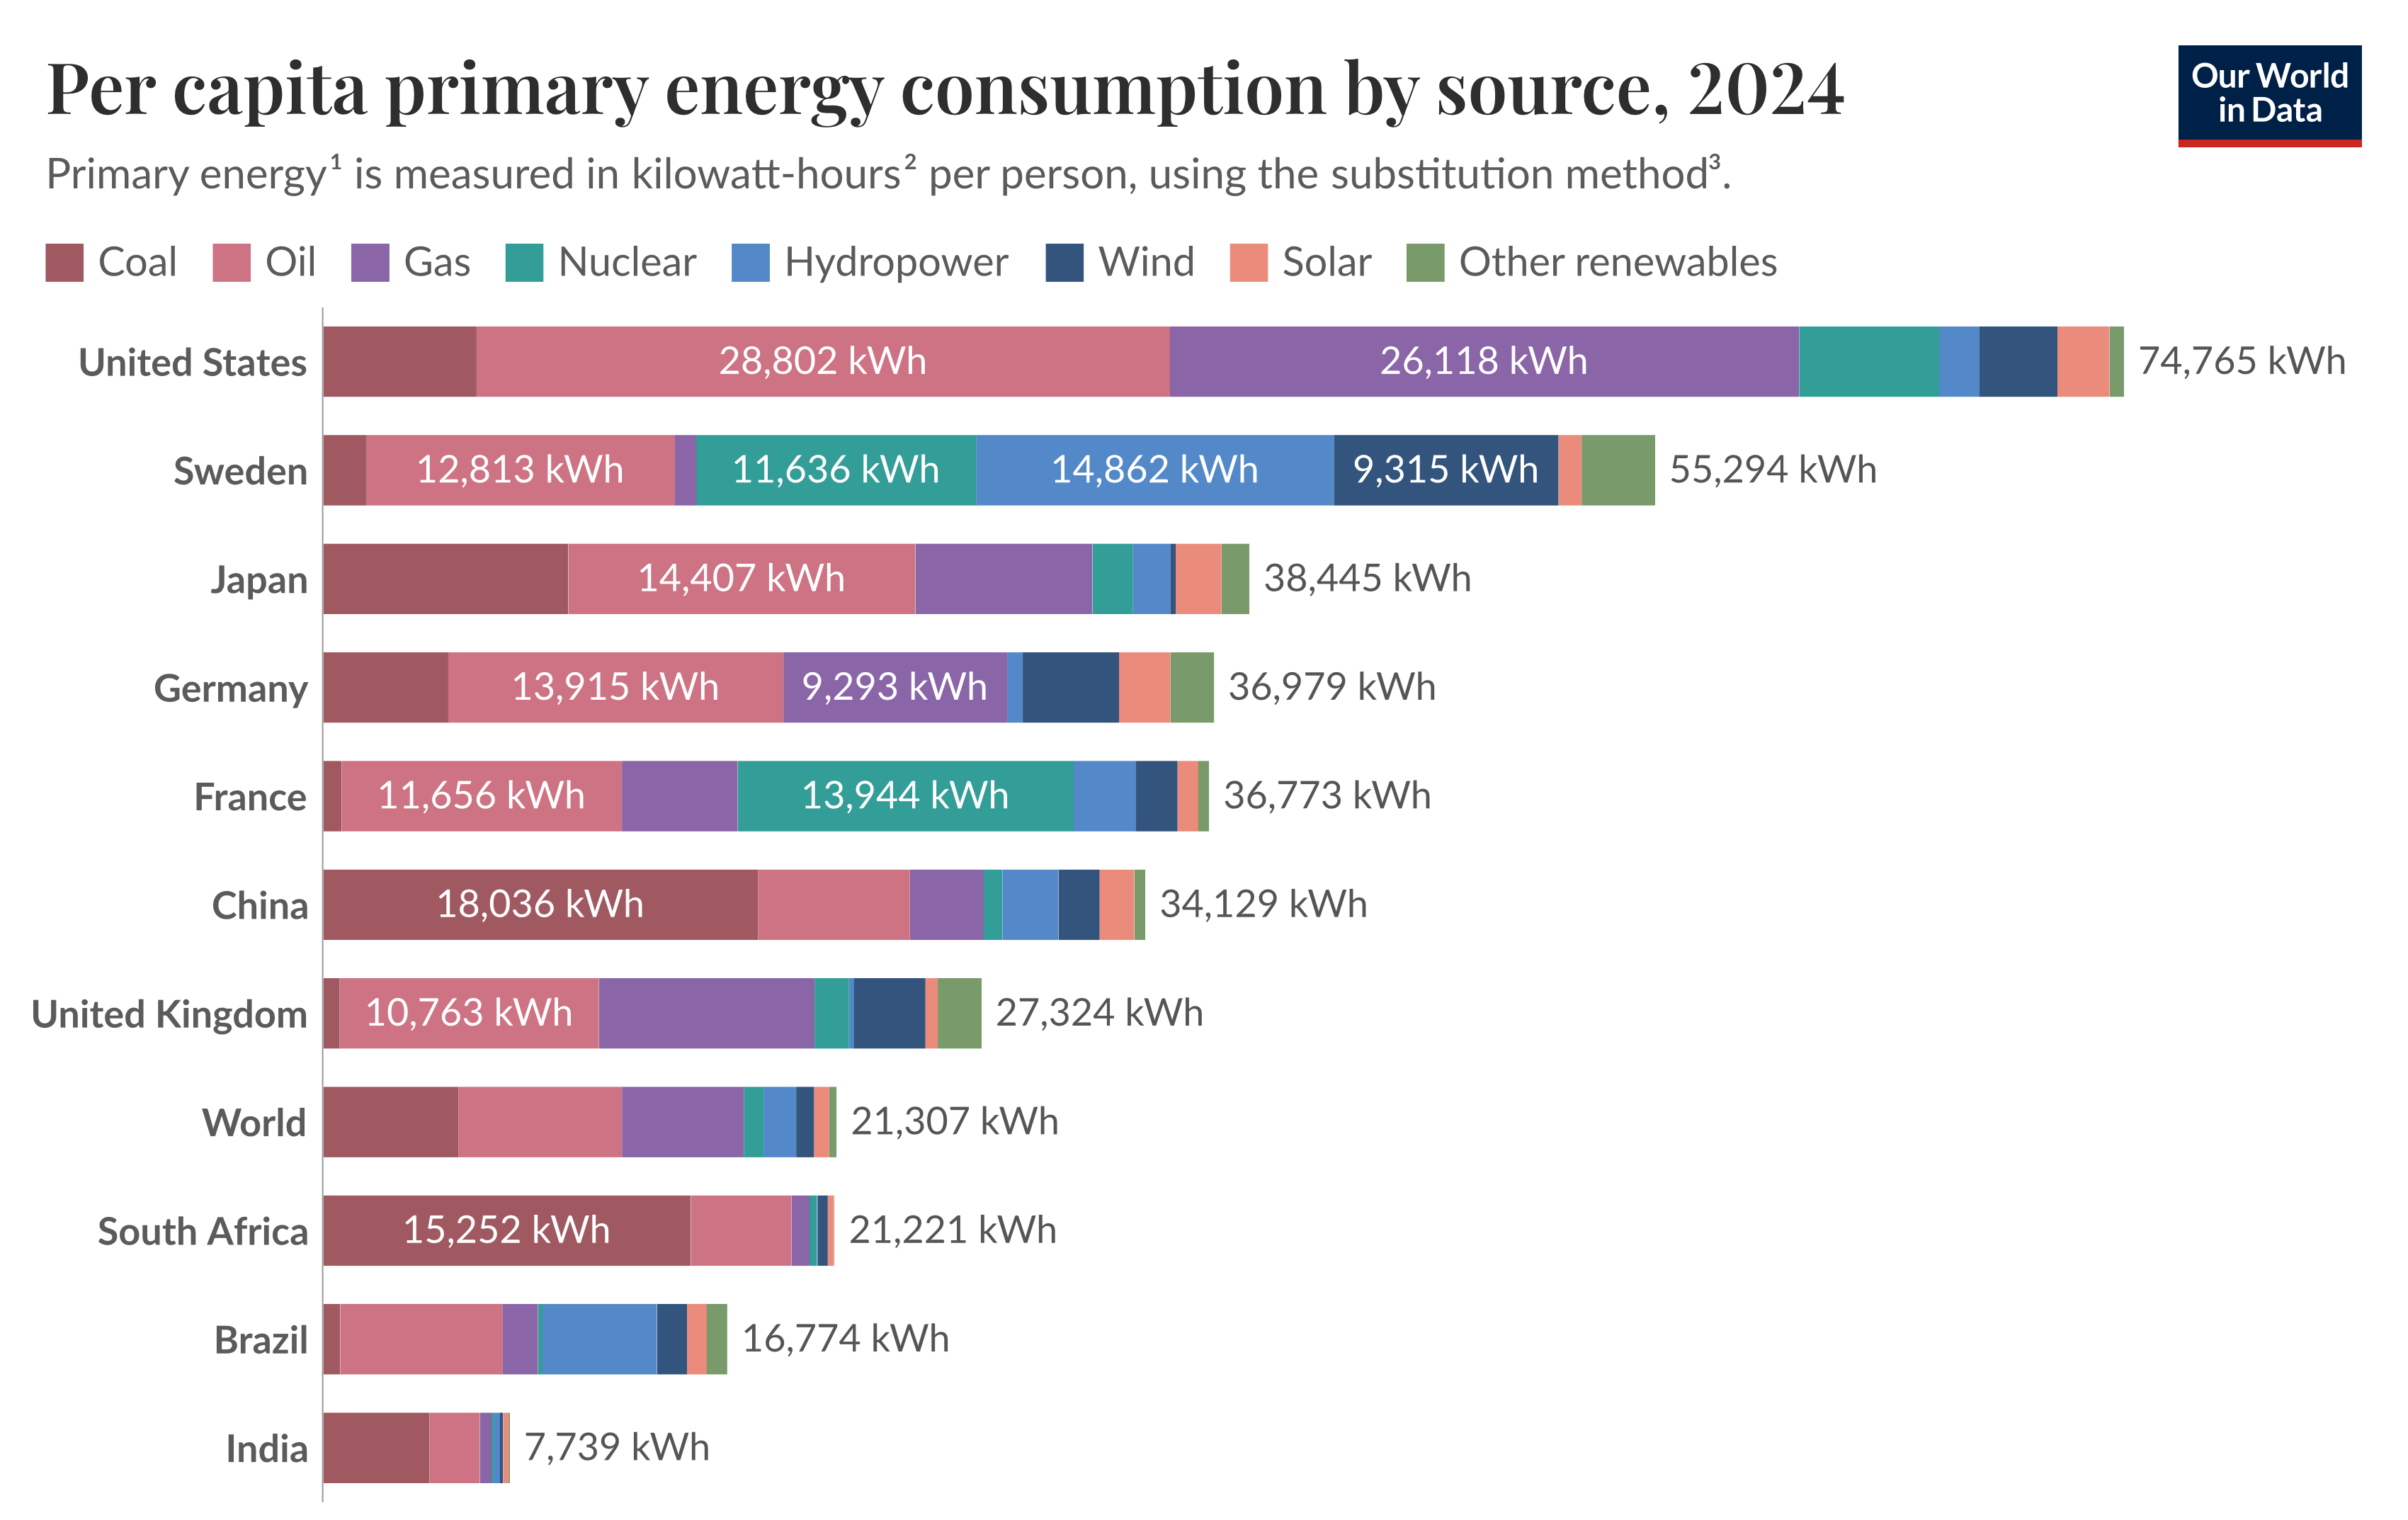
\includegraphics[width=\linewidth]{figures/per-capita-energy-stacked.png}
    \caption{Global primary energy consumption by source in 2024; source: \href{https://ourworldindata.org/energy-production-consumption}{Our World In Data}}
    \label{fig:energy_consumption_2024_percapita}
\end{figure}

Figure \ref{fig:energy_consumption_2024_percapita} presents the global primary energy use per capita in 2024 \cite{EnergyUsePerson}. Primary energy refers to energy in its raw, untransformed state, as extracted from natural resources. This includes, for example, coal prior to combustion, crude oil before refining, natural gas before processing, and uranium before enrichment\footnote{Following \href{https://ourworldindata.org}{Our World In Data}'s definition \cite{ritchieEnergyMix2020}, primary energy encompasses the total energy content of energy resources before conversion into secondary forms such as electricity, district heat, or refined fuels. It therefore includes both the energy ultimately delivered to end users and the losses and inefficiencies associated with transformation, transmission, and distribution processes.}.

Historical data indicate that global primary energy consumption has increased almost continuously over the past five decades, as shown in \Cref{fig:energy_trend_per_captia}. Notable exceptions include temporary declines in the early 1980s, during the global financial crisis in 2009, and in 2020 as a result of the COVID-19 pandemic. Although total energy consumption continues to rise, the growth rate appears to be stagnating, currently averaging approximately 1–2\% per year.

\begin{figure}[ht]
    \centering
    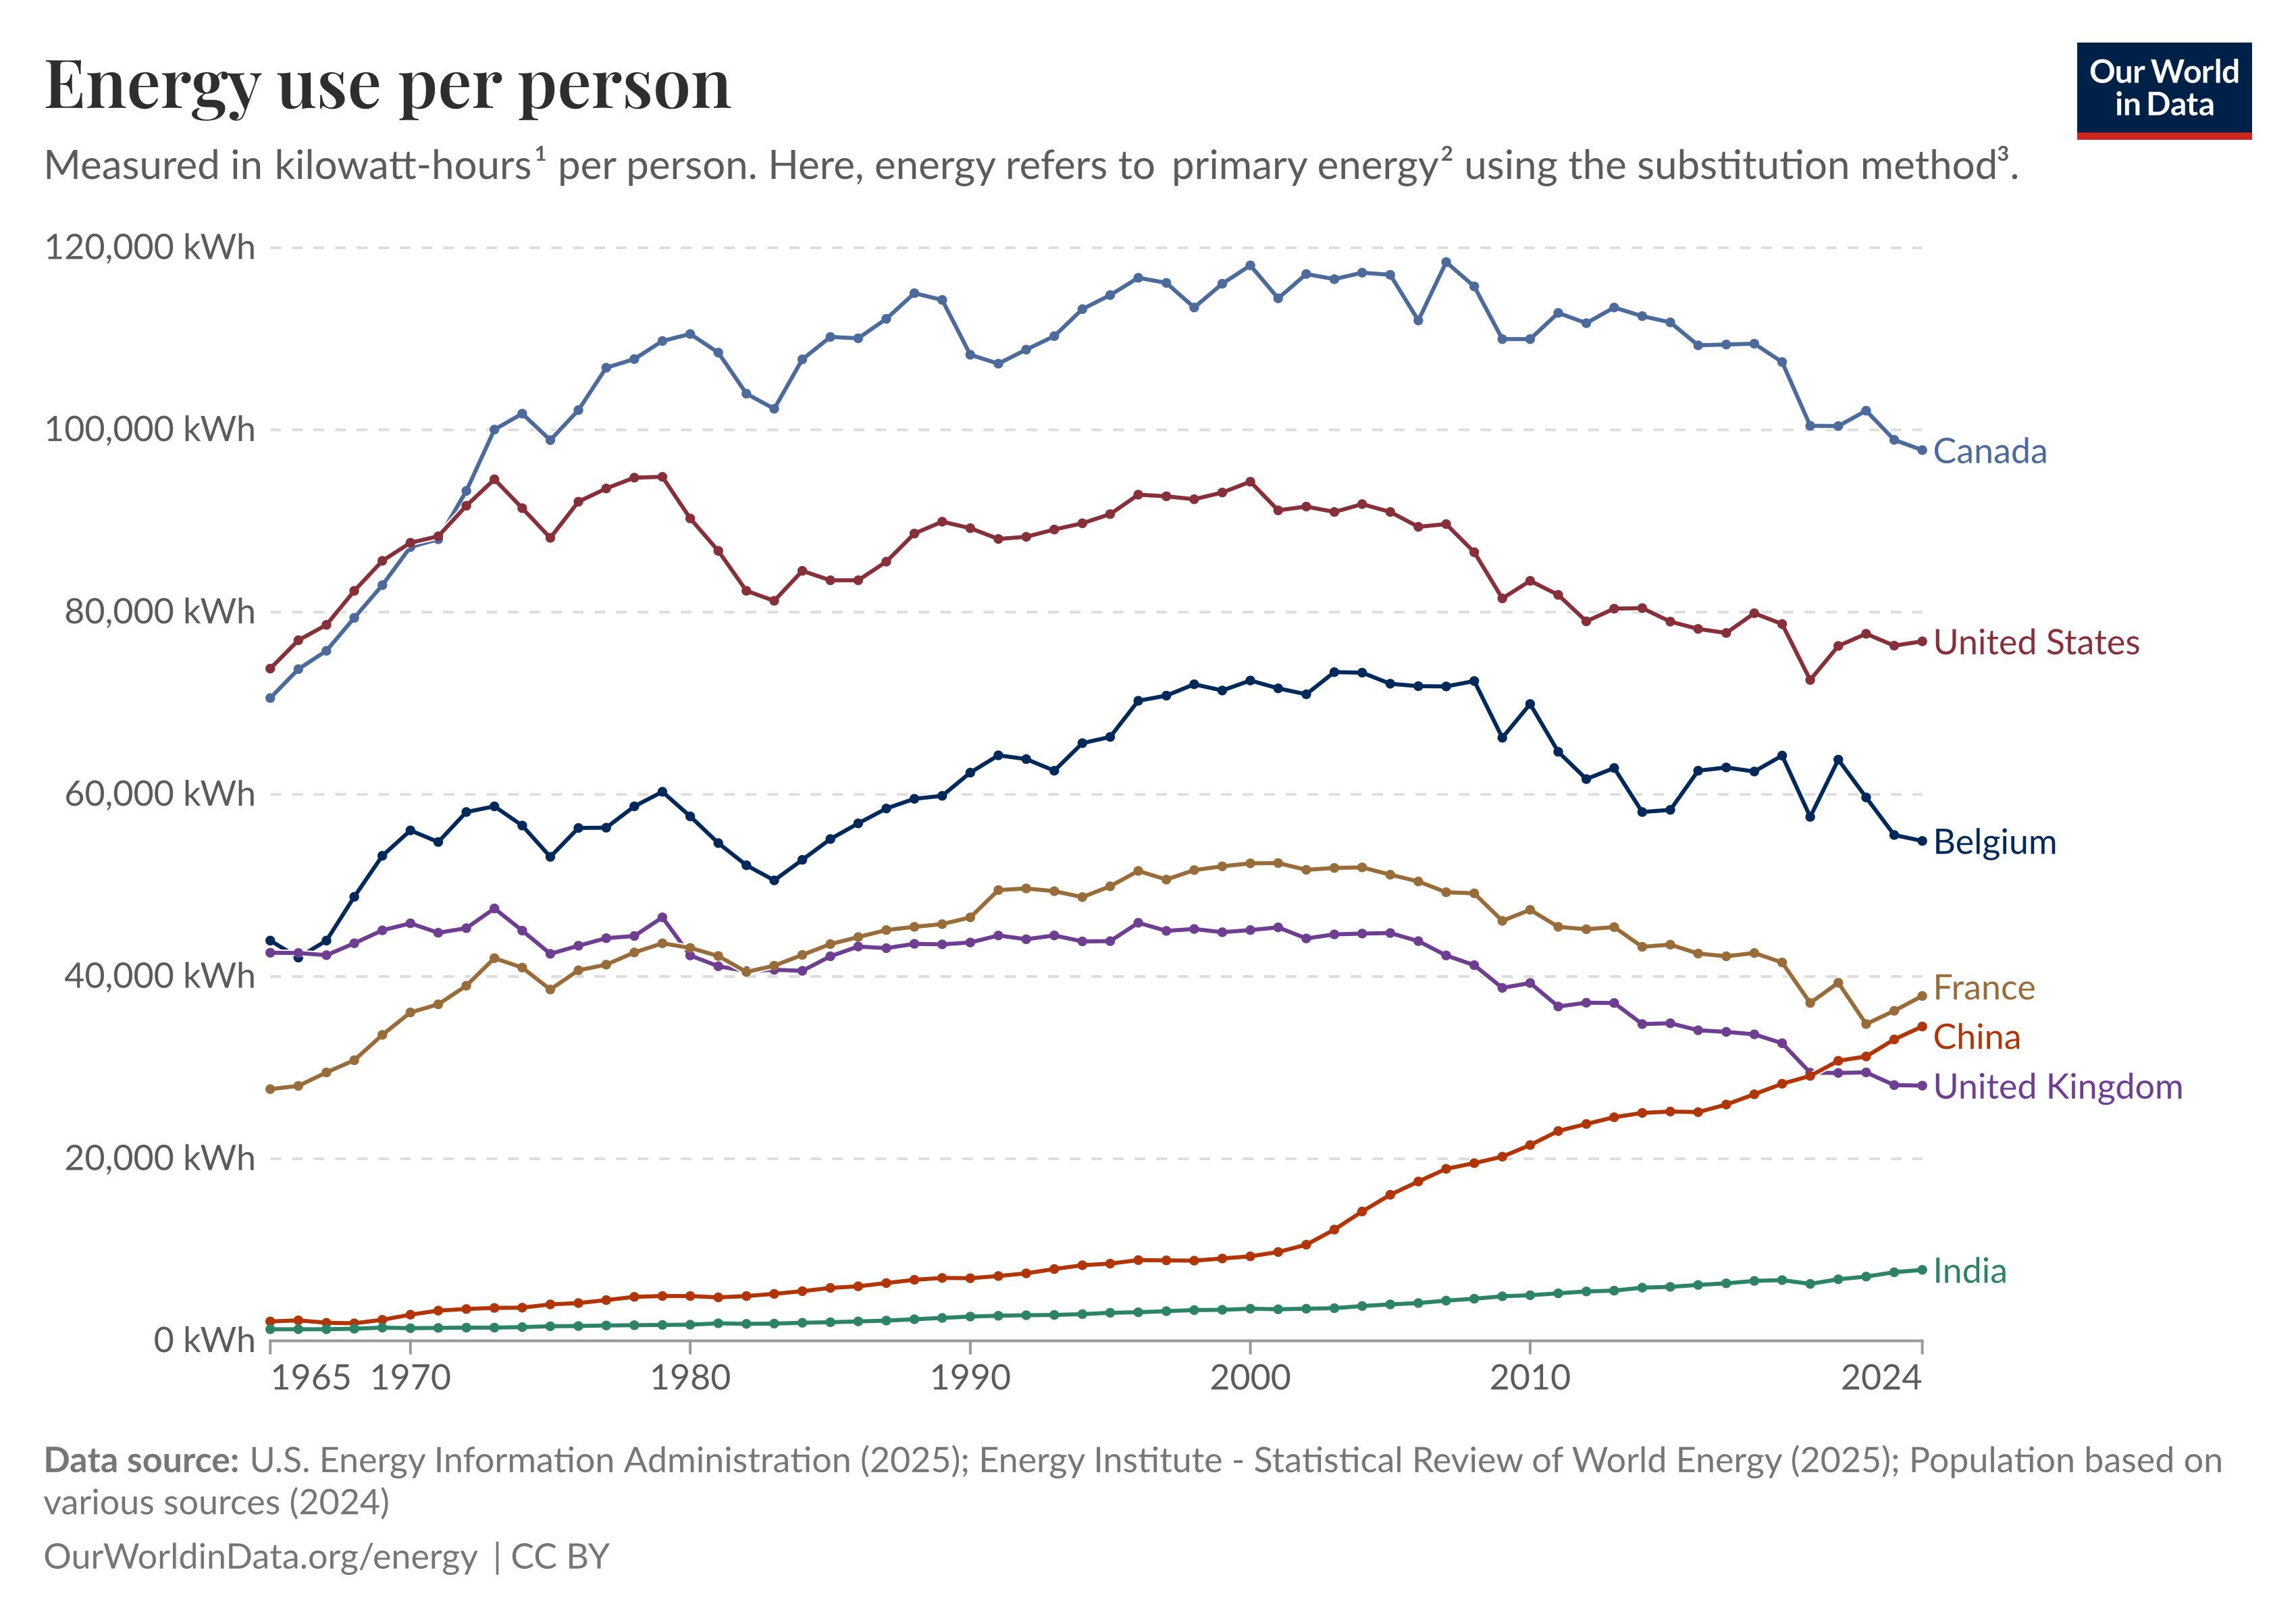
\includegraphics[width=0.8\linewidth]{figures/per-capita-energy-use-2.png}
    \caption{Per capita share of energy in 2024; source: \href{https://ourworldindata.org/energy-production-consumption}{Our World In Data}}
    \label{fig:energy_trend_per_captia}
\end{figure}
Overall, these trends reflect a structural increase in global energy demand, largely driven by population growth, economic \& technological development, and rising living standards in many regions. From an engineering perspective, this sustained demand growth reinforces the importance of designing energy systems that are not only efficient and reliable, but also sustainable and resilient in the context of climate and resource constraints.

% Energy is the fundamental ability to do work. We all need energy. Energy is increasingly becoming an important topic of discussion, in part due to the energy transition, but also due to the growing energy consumption.
% Cref{fig:x} shows the primary energy use per person in the world in 2024. The primary energy use refers. (World data defines primary energy as the energy that is available as resources – such as the fuels burnt in power plants – before it has been transformed. This relates to the coal before it has been burned, the uranium before it has been refined, or the barrels of oil before it has been processed. Primary energy includes energy that the end user needs, in the form of electricity, transport and heating, plus inefficiencies and energy that is lost when raw resources are transformed into a usable form.) (cite{world data}. We see that global energy consumption has increased nearly every year for more than half a century. The exceptions to this are in the early 1980s, 2009 following the financial crisis, and 2020 due to the COVID-19 pandemic.
% Global energy consumption continues to grow, but the growth does seem to be slowing down—averaging around 1\% to 2\% per year.
% Thus, we see that the demand for energy is growing across many countries in the world, as people get richer and populations increase.

\subsection{Energy Mix}
Figure \ref{fig:global_energy_shares} illustrates the global distribution of primary energy consumption by source and shows a rapid increase in energy consumption from the 20th century onwards. Oil remains the dominant contributor to the global energy mix, followed by coal and natural gas, with hydroelectric power representing a smaller but still significant share. Although modern renewable energy sources (\hyperref[sec:renewable_energy]{RES})—such as wind and solar—currently account for a comparatively modest fraction of total primary energy use, their growth rates over the past decade have been substantial.

% From ref{fig} we see that globally we get the largest amount of our energy from oil, followed by coal, gas, and hydroelectric power. Although renewable make for a very small amount compared to the other energy sources, they are now growing quickly. Ref{fig} shows a chart with the specific breakdown by source, including coal, gas, oil, nuclear, hydro, solar, wind, and other renewables (which include bioenergy, wave, and tidal). This is given in terms of per capita consumption. Here it is also clear that global trends tend towards the same conclusion: energy demand is rising.

\begin{figure}[ht]
    \centering
    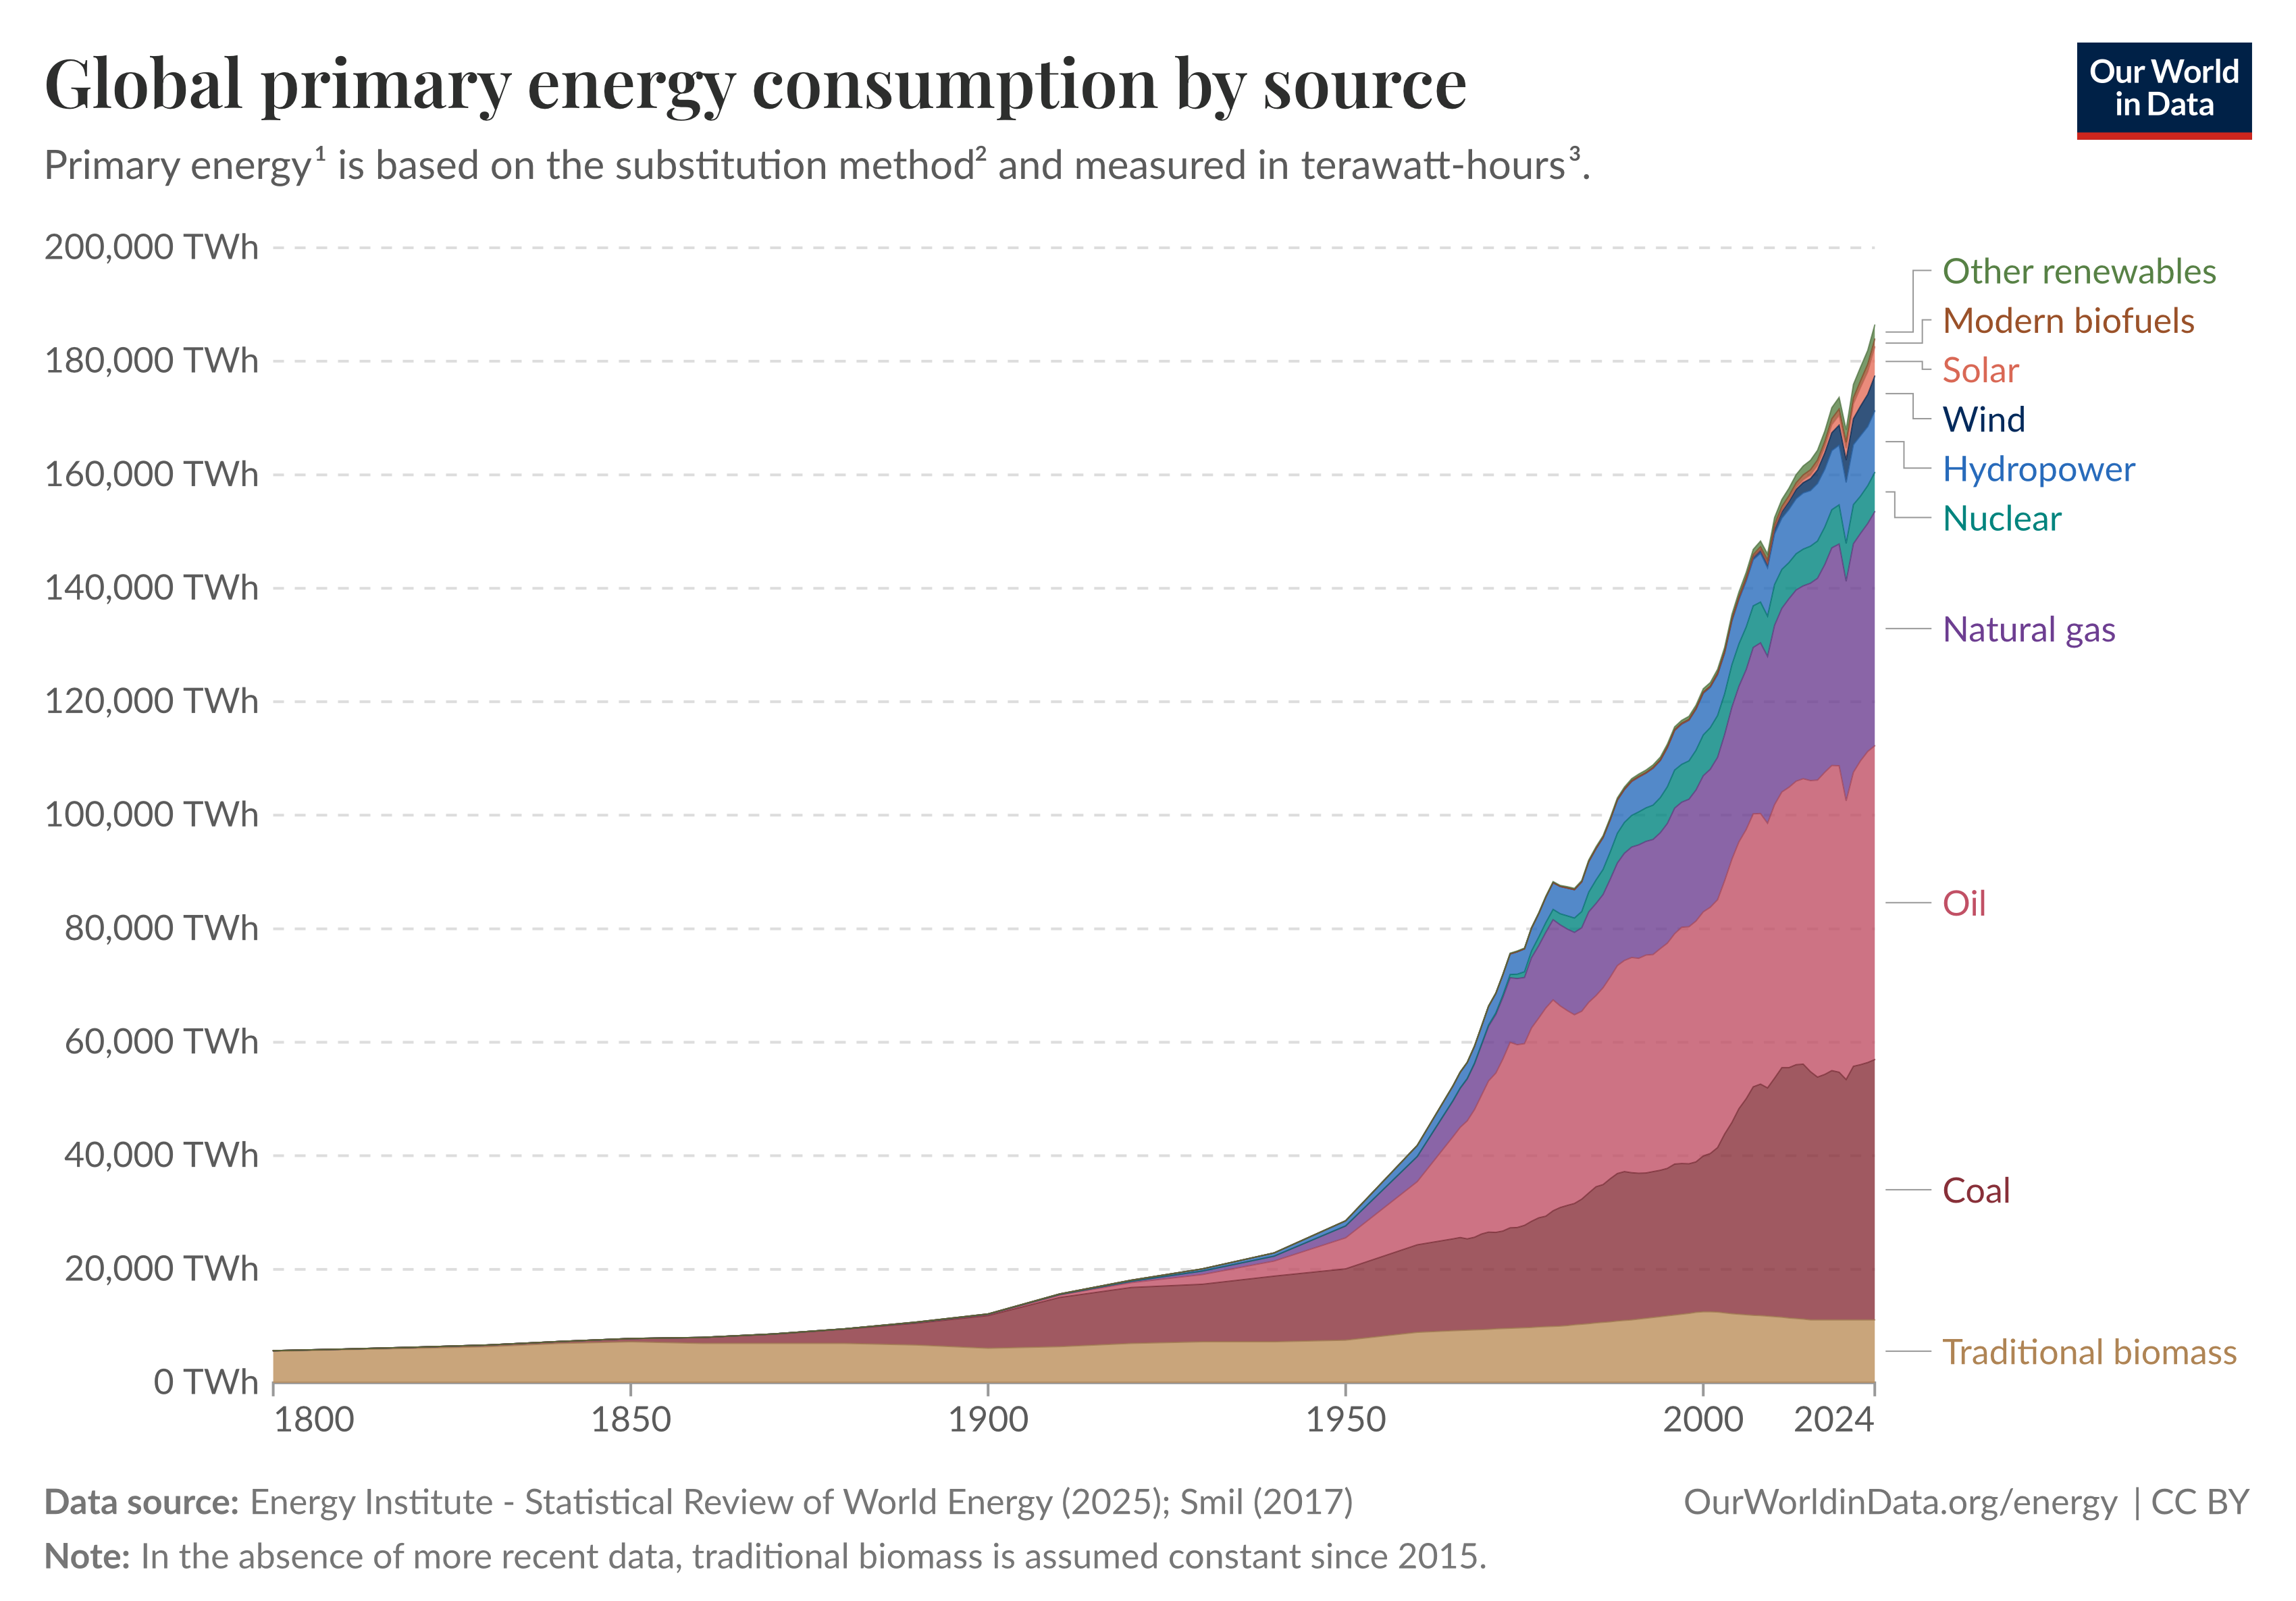
\includegraphics[width=0.85\linewidth]{figures/global-energy-substitution.png}
    \caption{Different sources of global energy use over the years; source: \href{https://ourworldindata.org/energy-mix}{Our World In Data}}
    \label{fig:global_energy_shares}
\end{figure}


\subsection{Electricity Mix}\label{sec:electricity_mix}
The electricity mix constitutes a specific subset of the broader energy mix. While the overall energy mix includes all primary energy uses—such as transport fuels, industrial heat, and residential heating—the electricity mix refers exclusively to the energy sources used to generate electrical power. In other words, it represents the composition of fuels and technologies that supply the grid and ultimately power households, industry, digital infrastructure, and electric vehicles (EVs) \cite{EnergyMix2025}. Consequently, the relative shares of coal, oil, natural gas, nuclear energy, and renewable sources differ between the total energy mix and the electricity mix.

The line chart in Figure \ref{fig:elec_mix_share_by_source} illustrates the evolution of each source’s share in global electricity generation over time. Globally, coal remains the dominant source of electricity generation, followed by natural gas. Among low-carbon sources, hydropower and nuclear energy historically contribute the largest shares, although wind and solar power have experienced rapid growth in recent years and are increasingly significant contributors to new capacity additions \cite{RenewableElectricityRenewables}.

\begin{figure}[ht]
    \centering
    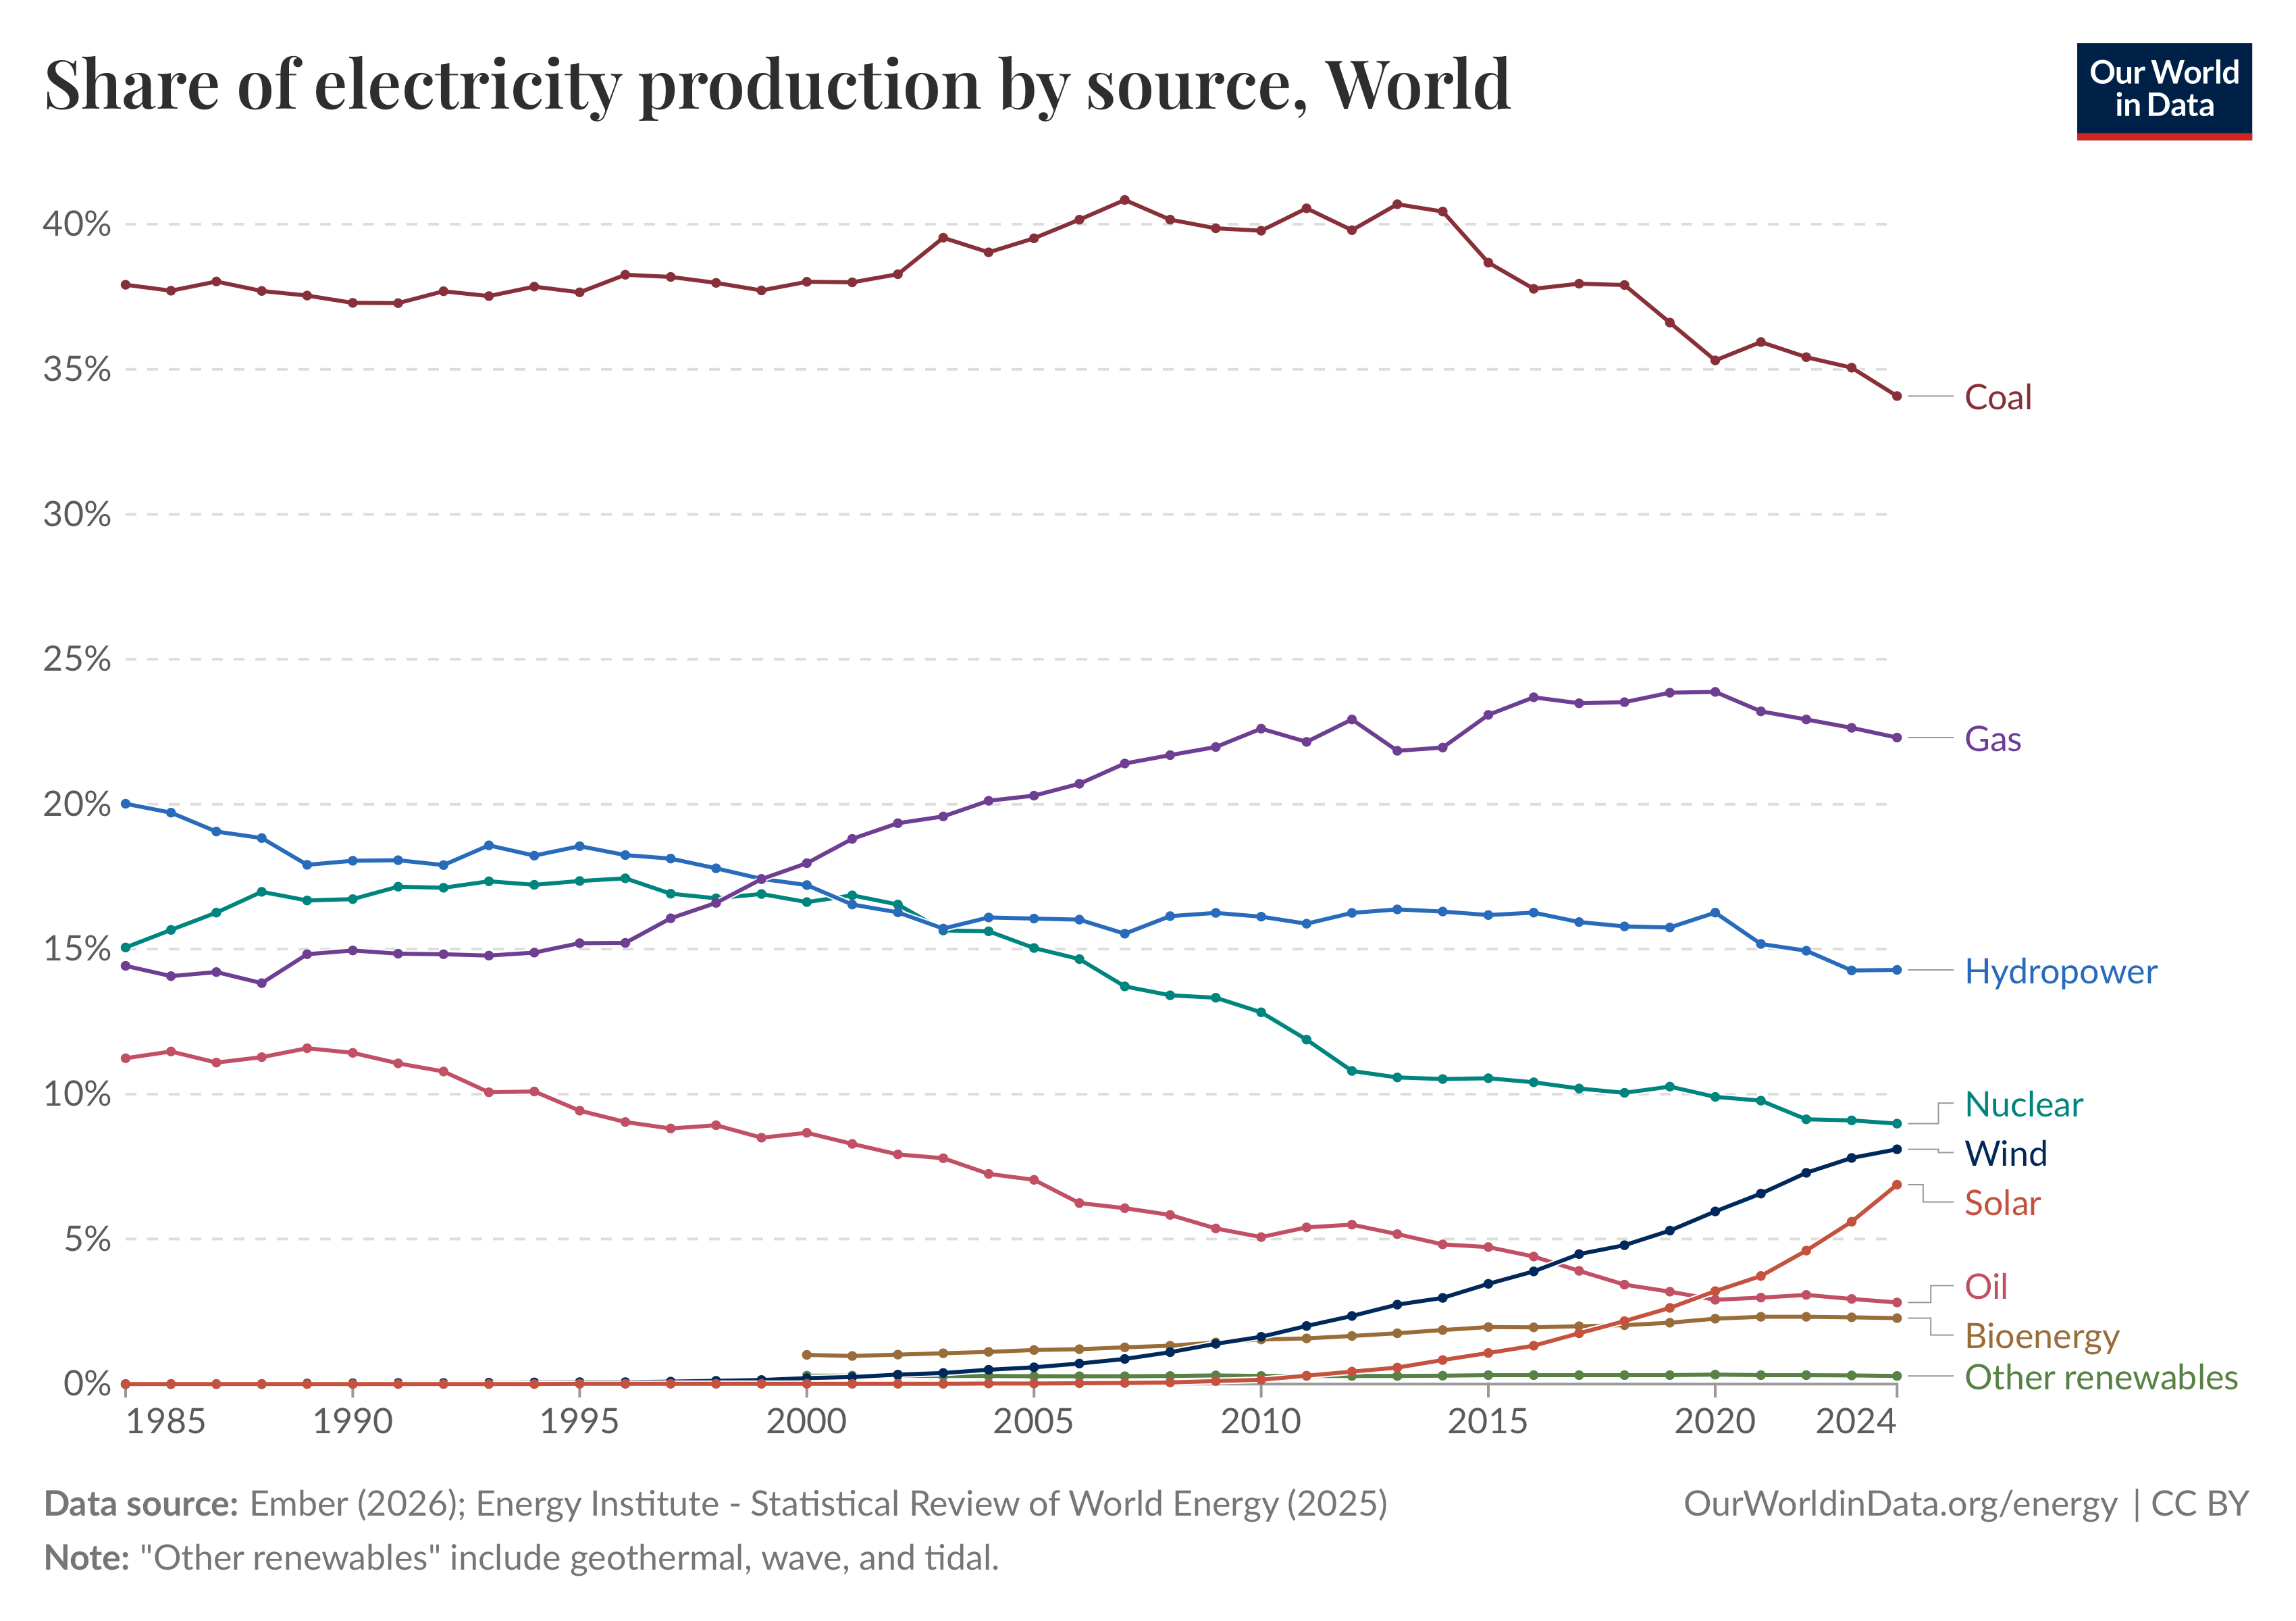
\includegraphics[width=0.7\linewidth]{figures/share-elec-by-source.png}
    \caption{Different shares of electricity production by source throughout time; source: \href{https://ourworldindata.org/electricity-mix}{Our World In Data}}
    \label{fig:elec_mix_share_by_source}
\end{figure}

\subsubsection*{Belgian electricity mix}
The Belgian electricity mix exhibits a markedly different structure. As shown in Figure \ref{fig:BE_elec_share}, approximately 28\% of electricity generation is derived from fossil fuels, while around 33\% originates from nuclear power. RES—particularly wind and solar—account for a substantial and growing share of generation. This national profile reflects how electricity mixes can vary significantly across countries despite similar overarching decarbonization objectives.

\begin{figure}[ht]
    \centering
    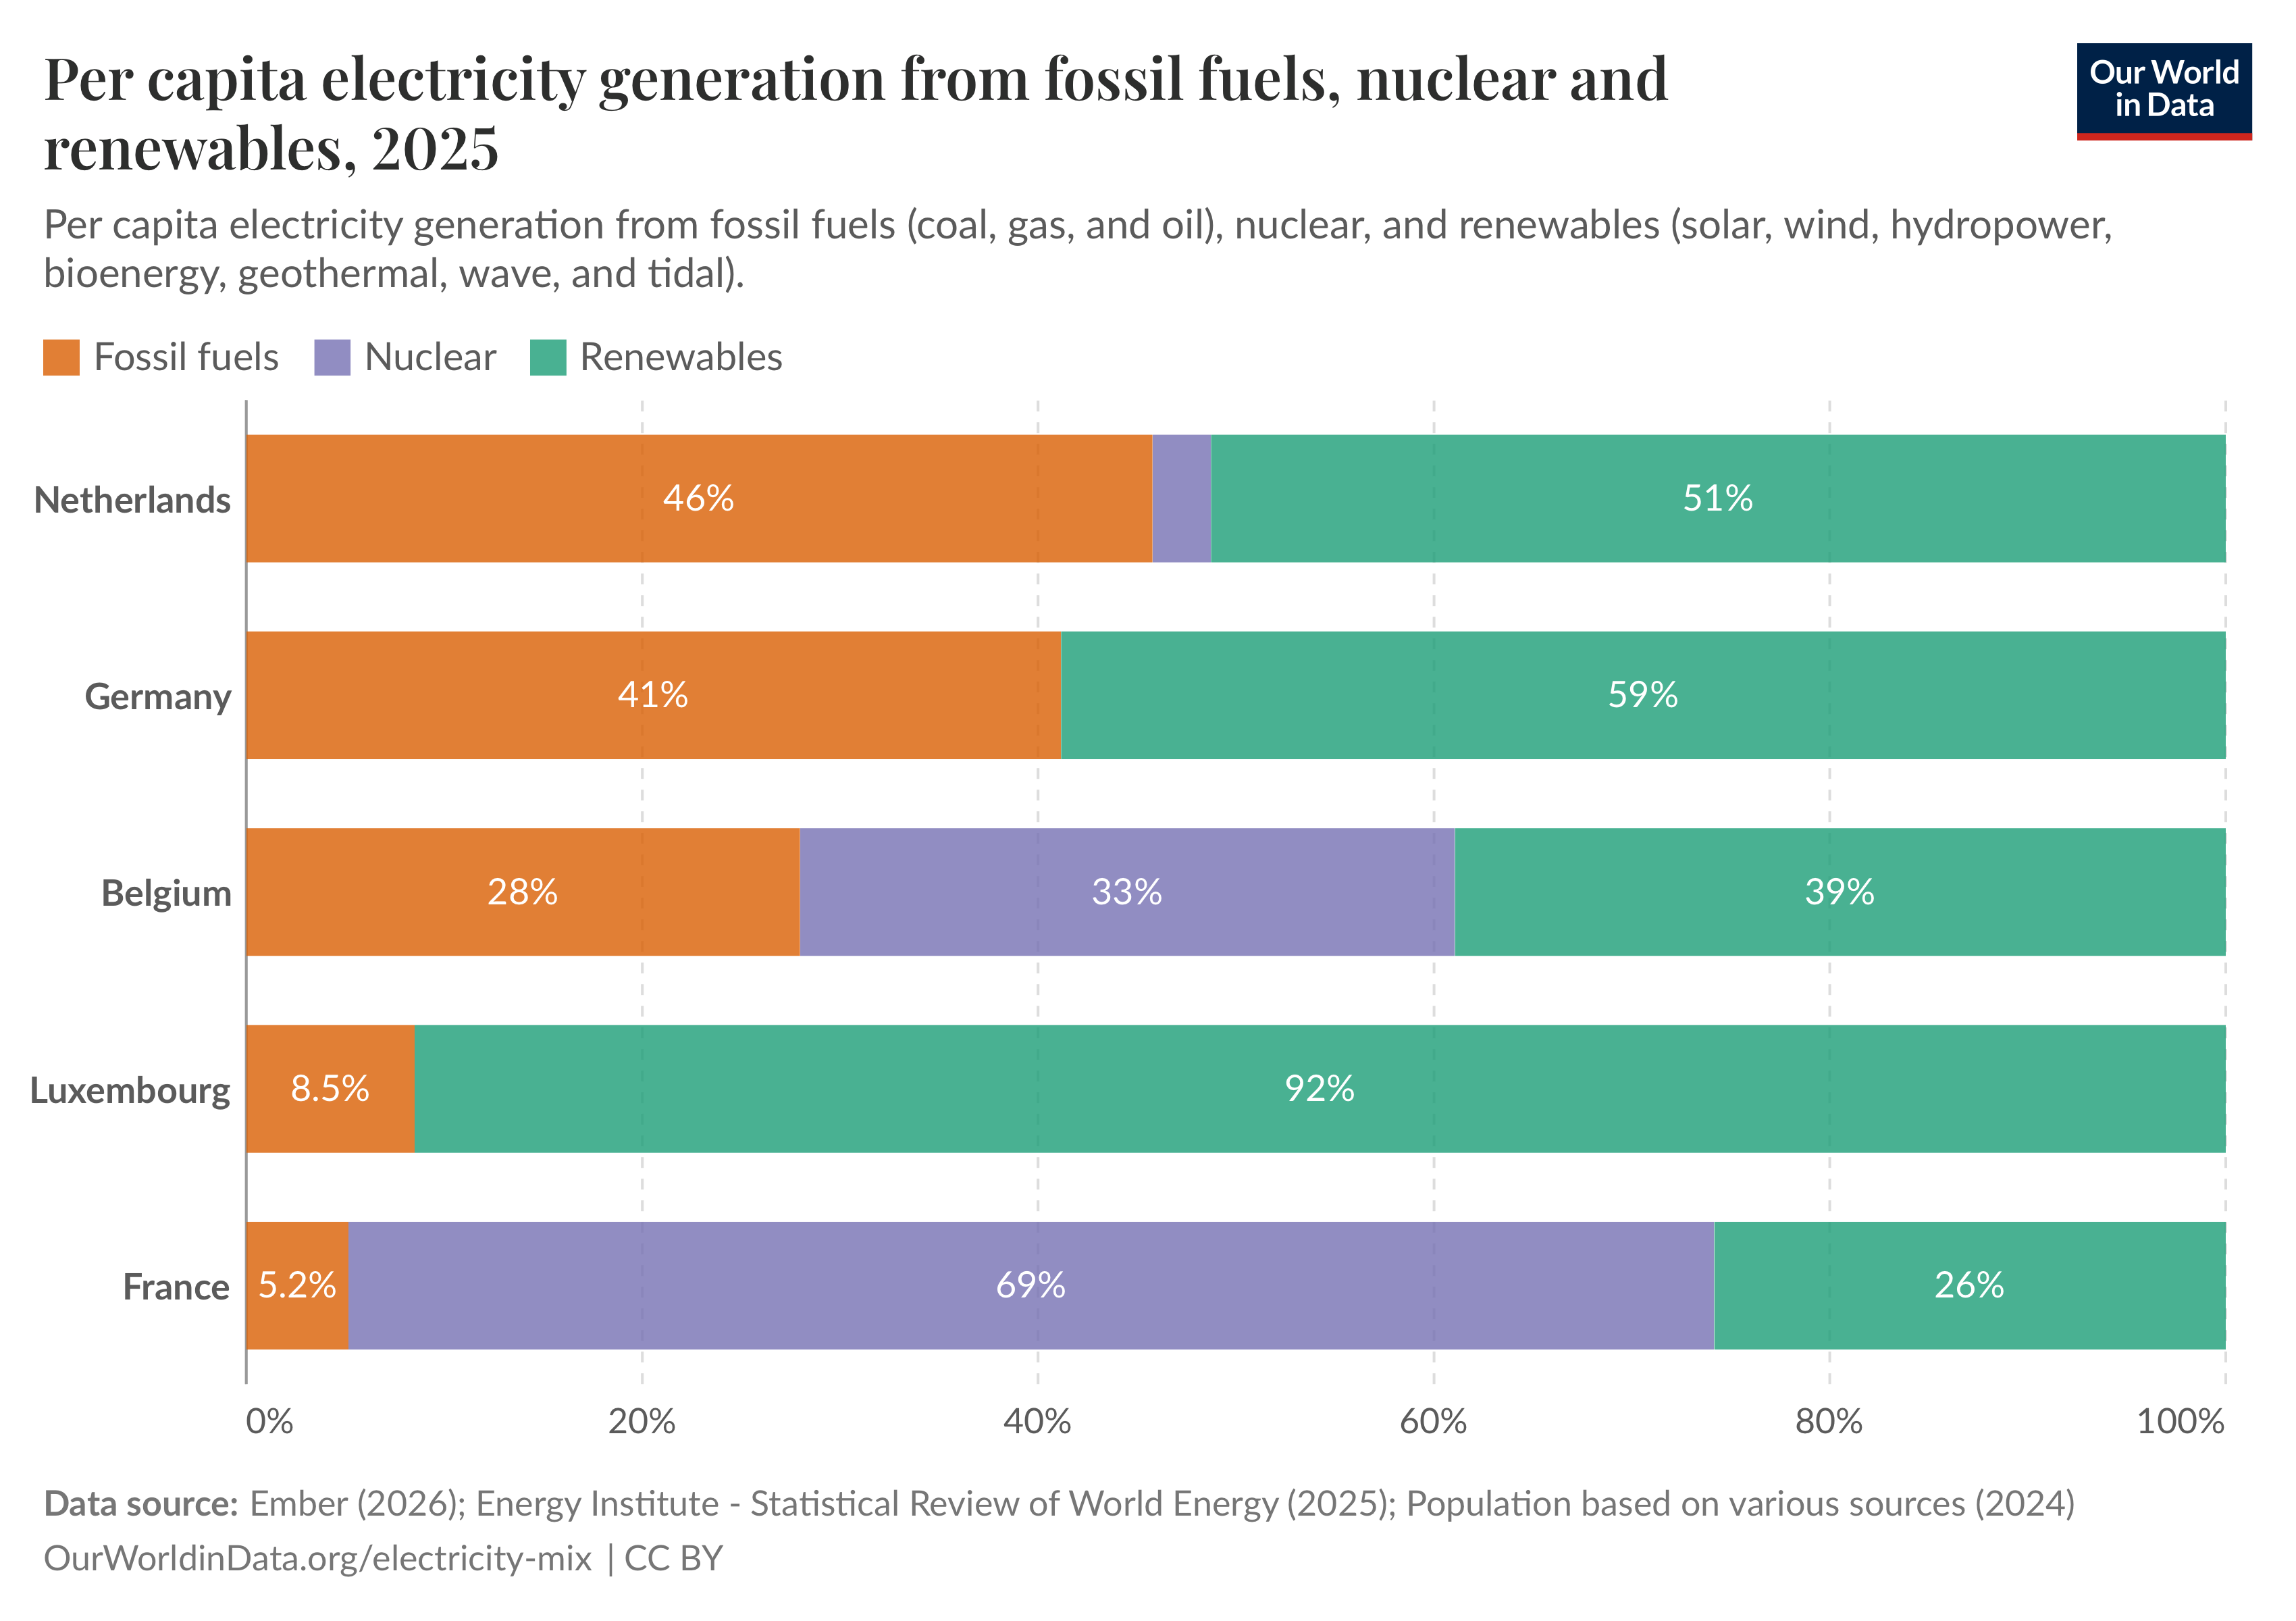
\includegraphics[width=0.8\linewidth]{figures/per-capita-electricity-fossil-nuclear-renewables.png}
    \caption{Share of electricity in Belgium compared to the neighbouring countries; source: \href{https://ourworldindata.org/electricity-mix}{Our World in Data}}
    \label{fig:BE_elec_share}
\end{figure}


\subsection{Renewable Energy}\label{sec:renewable_energy}
Renewable energy is power generated from natural sources that replenish on a human timescale, such as the sun, the wind, water, and heat from the earth. These sources are used to produce electricity and heat with significantly lower greenhouse gas (GHG) emissions\footnote{The \href{https://www.ipcc.ch}{IPCC} formally describes GHG emissions as gaseous components of the atmosphere that absorb and emit radiation at specific wavelengths within the spectrum of radiation emitted by the Earth’s surface, by the atmosphere itself, and by clouds. This traps heat, keeps the earth warm, and is called the greenhouse effect \cite{FrequentlyAskedQuestions}.} compared to fossil fuels, making them vital for addressing climate change and air pollution \cite{RenewableEnergyEESI}.

\subsubsection*{Technology \& deployment}
Common technologies include photovoltaic (PV) panels, wind turbines, water dams, and geothermal heat pumps. \Cref{fig:conversion_techs} shows a summary of those technologies paired with their possible energy sources. The main technologies studied for this thesis are PV panels and heat pumps, as they are the most relevant to the scope of residential energy modelling (\Cref{sec:residentialTechnologies}).

\begin{figure}[ht]
    \centering
    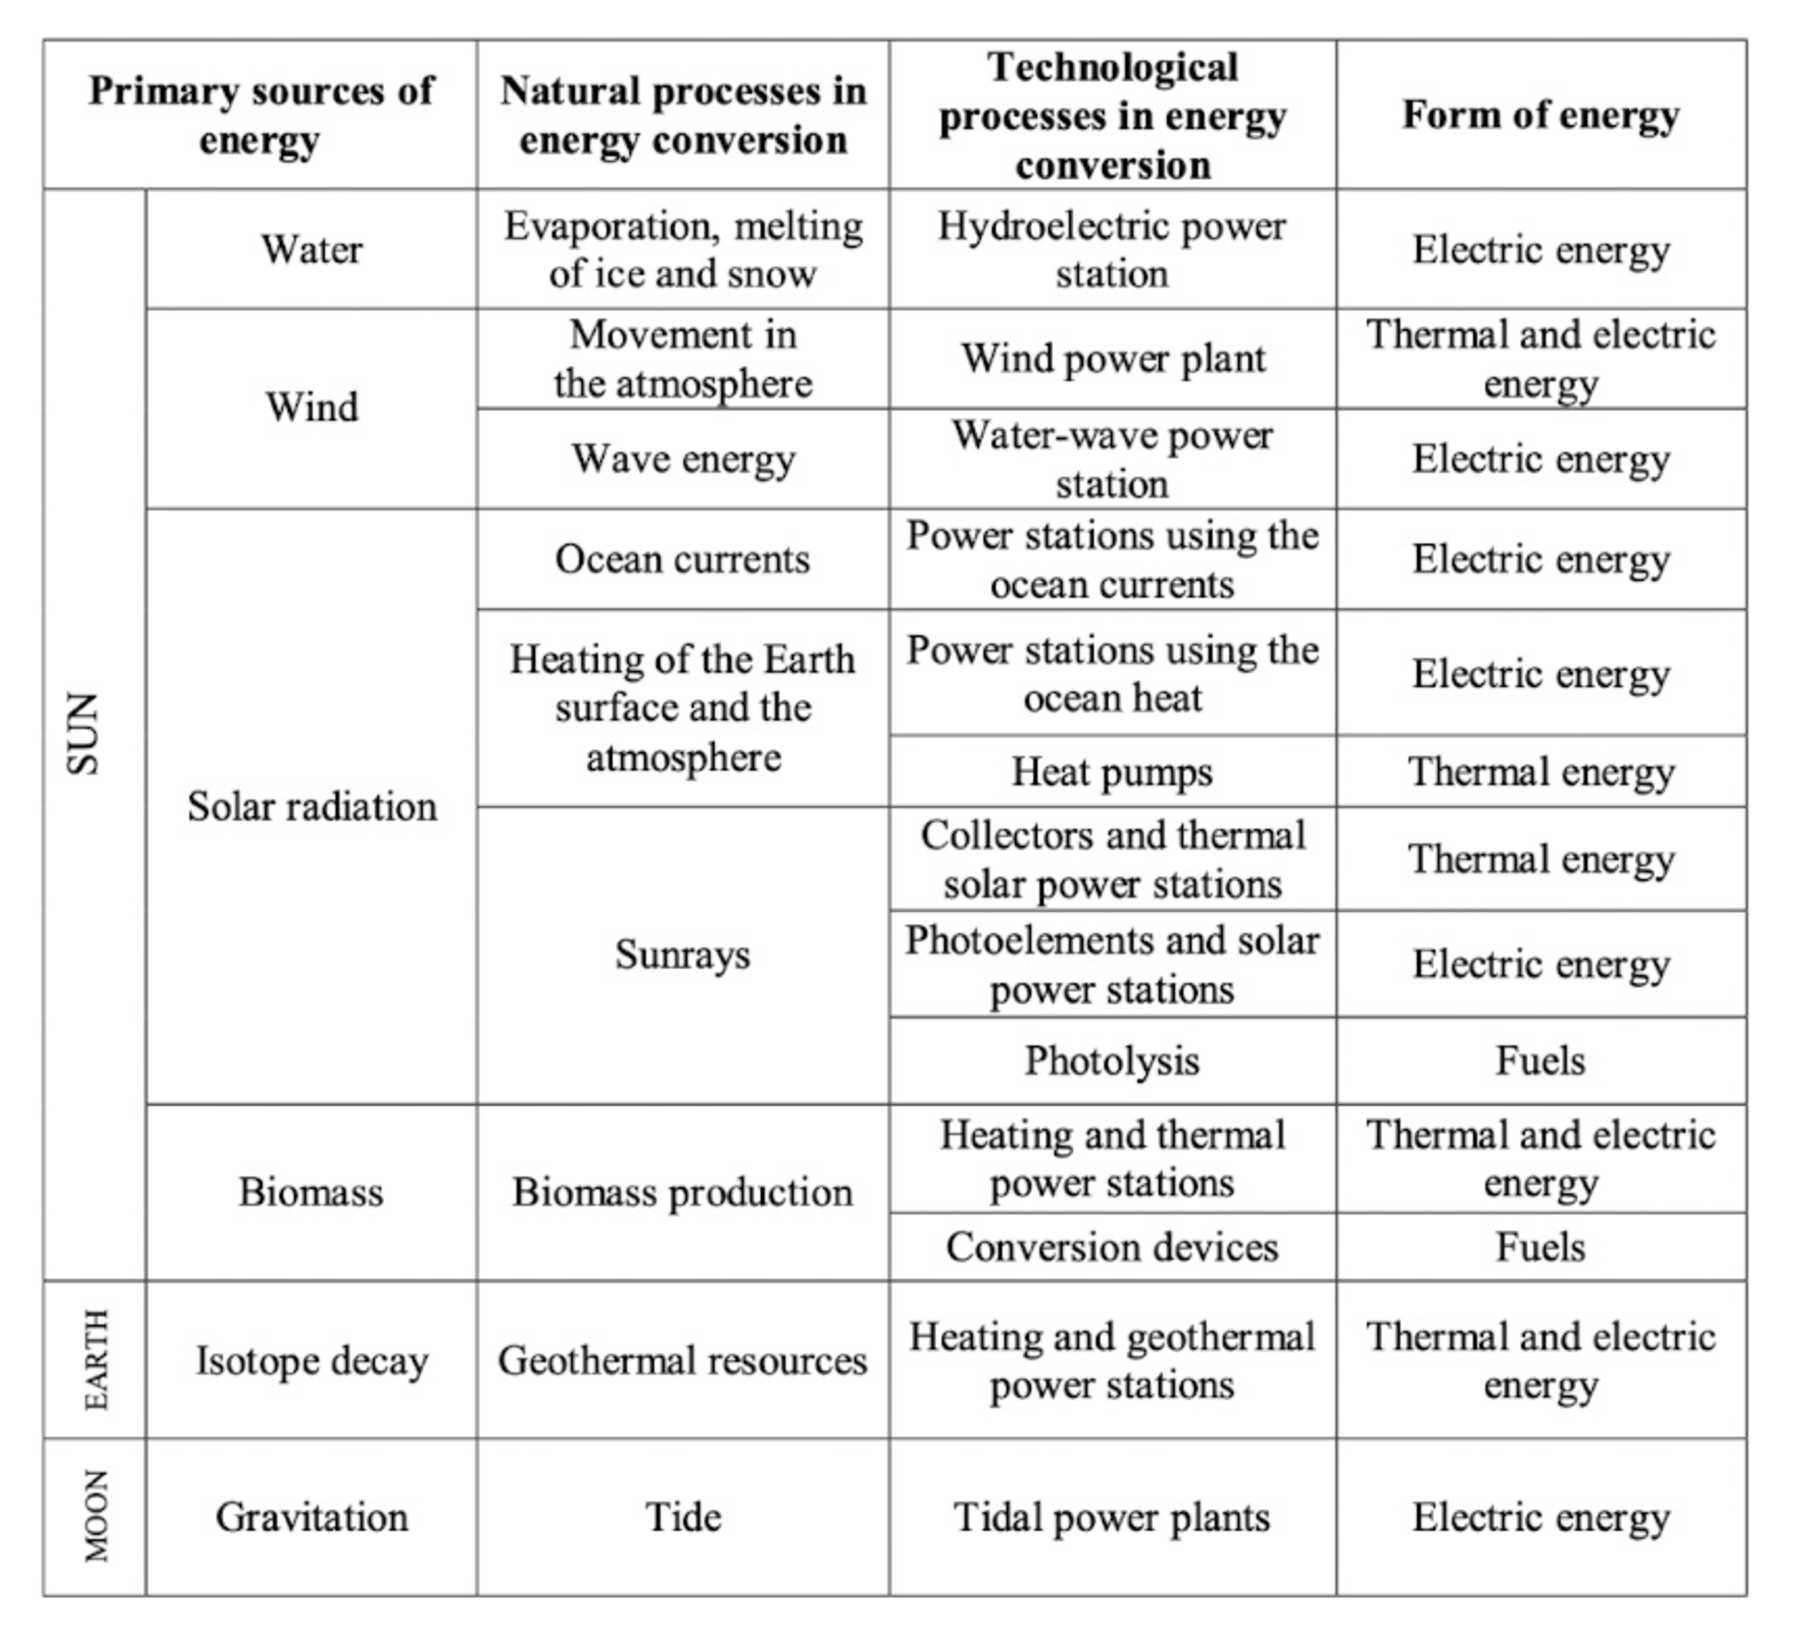
\includegraphics[width=0.8\linewidth]{figures/conversion_tech.pdf}
    \caption{Division of renewable energy sources and the possibilities of conversion, adapted from Zielińska~\cite{zielinska2010_sustainable_development} by Prof. Svend Bram.}
    \label{fig:conversion_techs}
\end{figure}

\subsubsection*{Sustainability}
Renewables are closely linked to sustainable energy—but they are not quite the same thing. The term ``sustainability'' refers to a society's ability to exist, develop, and meet the needs of the present without compromising the ability of future generations to meet their own needs and develop. Sustainability goes further than only the energy supply. It includes environmental, economic and social dimensions. 

\subsubsection*{Decarbonisation}
The relevance of renewable energy follows directly from the energy system's dominant role in global warming: roughly 73\% of global anthropogenic GHG emissions originate from energy production and use \cite{intergovernmentalpanelonclimatechangeipccEnergySystems2023}. Any credible mitigation strategy must therefore target the decarbonisation of energy systems first.
\newline Renewable technologies meet this challenge by replacing carbon-intensive carriers with low- or zero-emission alternatives. Solar and wind generate electricity without combustion-related emissions, while hydropower and geothermal provide relatively stable low-carbon supply. Raising the renewable share is thus a necessary condition for reducing emissions at scale—the rationale underpinning frameworks such as the European Green Deal, which targets climate neutrality by 2050 through a large-scale transformation of the energy system \cite{EuropeanGreenDeal}.

\subsubsection*{Reduction \& reconstruction of energy demand}
The transition cannot be framed solely as expanding clean supply. Global energy demand is still rising—driven by population growth, economic development, and digitalisation—so renewables must both displace fossil generation and meet additional demand, sharply increasing the required deployment rate and system complexity \cite{ritchieEnergyMix2020}. This is the central limitation of a purely supply-driven view.
\newline Reducing and restructuring demand is therefore equally important. Lower total consumption shrinks the infrastructure needed for decarbonisation and eases pressure on resources, land use, and grid stability, while reshaping demand—through efficiency, behavioural change, and demand-side flexibility—improves alignment with variable generation. Better insulation cuts heating demand, and flexible consumption lets load follow renewable output, reducing the need for storage and balancing capacity. Demand reduction is, in this sense, a fundamental lever for making the transition technically and economically feasible.

\subsubsection*{Increasing RES}
Despite these challenges, renewable deployment has accelerated markedly. Although fossil fuels still dominate the primary energy mix, RES supplied roughly 8\% of global primary energy in 2023 and are projected to reach roughly 30\% of global primary energy by 2050 under current and announced policy trajectories \cite{iea2025weo}. This growth is driven mainly by falling wind and solar costs, supportive policy, and rising climate ambition at national and supranational levels.
\newline Integrating high RES shares generally requires a broader portfolio of balancing options—storage, transmission expansion, demand-side response, sector coupling, curtailment management, improved forecasting, synchronous condensers, and advanced inverter controls such as fast frequency response and grid-forming functionality. Robust electricity-demand modelling becomes correspondingly valuable: the better operators understand when, where, and how strongly demand evolves, the more effectively they can integrate renewable generation while preserving reliability and minimising curtailment and balancing costs \cite{entsoe_flexibility_res_2025, iea_value_demand_flexibility_2025}.

\paragraph{Merit order.} 
Variable RES reshapes power-system operation through the merit order. In liberalised markets, units are dispatched in ascending order of marginal cost \cite{PowerExchangeMarkets}; because wind and solar have near-zero marginal cost, they shift the merit order rightward, displacing costlier conventional plants and lowering wholesale prices when renewable output is high. This \textit{merit-order effect} cuts short-term system costs but compresses revenues for dispatchable generation, weakening investment signals for firm capacity.

\paragraph{Duck curve.} 
At higher penetration, the same dynamic produces sharp temporal mismatches between generation and demand, captured by the \textit{duck curve}: low net demand during midday solar peaks, followed by steep evening ramps as solar fades. System flexibility requirements rise accordingly, calling for fast-response generation and storage.

\subsubsection*{Renewables--pros \& cons}
The expansion of renewable energy thus presents a set of structurally coupled advantages and challenges. On the one hand, RES enable deep decarbonisation, reduce marginal generation costs, and decrease dependence on imported fuels. On the other hand, their variability introduces operational complexity, including increased balancing requirements, price volatility, and potential adequacy concerns due to reduced revenues for dispatchable generation. These trade-offs do not represent fundamental limitations, but rather a shift in system design requirements—from fuel-based optimisation toward flexibility, coordination, and temporal alignment between supply and demand.

\subsubsection*{Renewables in Belgium}
The Belgian electricity mix, as shown earlier in Figure \ref{fig:BE_elec_share}, reflects both progress and structural constraints. While the share of renewable energy remains modest in absolute terms compared to some frontrunner countries, Belgium performs relatively well within its regional context. Neighbouring countries exhibit varying profiles: Germany and the Netherlands rely more heavily on fossil fuels alongside expanding renewable capacity, whereas France derives the majority of its electricity from nuclear power. Belgium’s energy system shares certain similarities with France in that nuclear energy has historically played a significant role in electricity generation \cite{NuclearPowerBelgium}. Figure \ref{fig:BE_elec_share} shows that in 2025, nuclear power accounted for approximately 33\% of Belgium’s electricity mix. Nevertheless, public concerns regarding nuclear safety and long-term waste management, combined with evolving policy decisions, have led to a gradual phase-out strategy\footnote{In recent years, five of Belgium’s seven nuclear reactor units have been decommissioned following increasingly stringent regulatory and political measures \cite{NuclearPowerBelgium}.} 

\subsubsection*{Is nuclear power sustainable?}
Nuclear energy is released from the atomic nucleus. Today's nuclear electricity is produced by fission, which harnesses the energy from splitting heavy nuclei to raise steam and drive a turbine\footnote{Electricity can also be generated by nuclear fusion, but this remains at the research stage \cite{WhatNuclearFusion2023}.}. It is not renewable, since it depends on a finite supply of uranium rather than a source replenished on a human timescale. Its sustainability is contested. Proponents and major bodies such as the IAEA present nuclear as a pillar of a sustainable future, citing its low-carbon life cycle and high energy density \cite{FiveReasonsClean2026}. Critics, including CAN Europe, argue it fails the criteria for a sustainable source given unresolved waste management and the environmental burden of resource extraction \cite{c.dascaluPOSITIONPAPERNuclear2024}. New projects are also notoriously slow (10–15 years) and expensive \cite{StorageDisposalRadioactive, CanNuclearPower}, which critics see as a poor fit for urgent 2030 targets relative to rapidly deployable renewables. Even so, nuclear is increasingly classified as sustainable within modern climate-policy frameworks: the EU taxonomy now lists it as a ``transitional'' sustainable activity, provided projects meet strict safety and waste-disposal standards \cite{EUTaxonomySustainable}.

\subsubsection*{Socio-political challenges}
While the technical feasibility of highly renewable electricity systems is well supported, the primary barriers to implementation are increasingly recognised as socio-political rather than engineering-related. Large-scale deployment of wind farms, solar parks, and transmission networks is often constrained by permitting delays, land-use conflicts, and public acceptance, reflecting competing interests around environmental protection, landscape aesthetics, and local community concerns. The transition is therefore governed not only by technological readiness but also by institutional capacity and governance structures \cite{IEA_NetZero2021, WorldBank_Minerals2020}.
\newline It also requires substantial restructuring of electricity markets and policy frameworks. High shares of variable renewables demand new mechanisms for valuing flexibility, adequacy, and system services that traditional market designs do not fully capture, while coordinating investment in transmission, storage, and demand-side flexibility adds complexity and requires long-term policy consistency. Decarbonisation is thus best understood as a socio-technical transformation, in which engineering solutions must be embedded within politically and socially viable pathways \cite{IEA_NetZero2021}.

\subsubsection*{Achieving 100\% renewable}
Substantial modelling shows that renewable-dominated electricity systems can, in principle, reach high reliability and adequacy \cite{Denholm2021, Brown2018, Zappa2019} by combining short- and long-term storage, demand response, transmission expansion, and advanced grid control. The traditional notion of ``baseload'' is correspondingly seen as outdated: modern systems need not continuously running plants but a portfolio of services—energy supply, reserve capacity, frequency regulation, and system strength—deliverable by a diverse mix of inverter-based resources and storage \cite{NREL_GFM2020}.
\newline Still, even where 100\% renewable systems are technically feasible, the broader consensus does not treat them as universally optimal. Many authoritative net-zero pathways adopt a hybrid approach \cite{IEA_NetZero2021, IEA_Nuclear2019}, pairing high renewable shares with firm low-carbon generation such as nuclear to cut system costs, land use, and reliance on long-duration storage. The ``renewables versus nuclear'' framing is thus largely a \textit{false dichotomy}: system design is better cast as a reliability-constrained optimisation in which different technology mixes meet demand under varying constraints. The most robust strategy is typically a diversified portfolio where renewables supply most energy and firm capacity—potentially including small modular reactors\footnote{SMRs are a smaller, more power-dense reactor type producing up to 300\,MW(e) per module \cite{SMRs2023}; ``modular'' refers to factory-built, transportable components, offering potential cost and time savings over conventional reactors.} (SMRs)—supports adequacy and resilience during prolonged low-renewable-output events.


\pagebreak
\section{Energy Demand}\label{sec:energy_demand}
Energy demand can be defined as the total quantity of energy consumed by households, industry, services, and public institutions to sustain economic and social activity. Whereas \textit{energy supply} refers to the production and provision of energy carriers, \textit{energy demand} represents the consumption side of the system—the aggregated load arising from residential lighting, industrial processes, transportation, data centers, and other end uses \cite{WhatEnergyDemand}. In this sense, demand constitutes the driving force of the energy system: it is the pull that determines how much energy must be generated.


\subsection{Global Energy Consumption}\label{sec:globalEnergyConsumpt}
Forecasting future global energy consumption is inherently complex and subject to significant uncertainty, as many dynamic factors are at play that greatly influence energy use. The IEA World Energy Outlook 2025 presents alternative scenario pathways rather than a single deterministic forecast, showing how future energy demand depends on policy choices, technology deployment, and efficiency improvements \cite{iea2025weo,iea2025gec}.
\begin{figure}[ht]
    \centering
    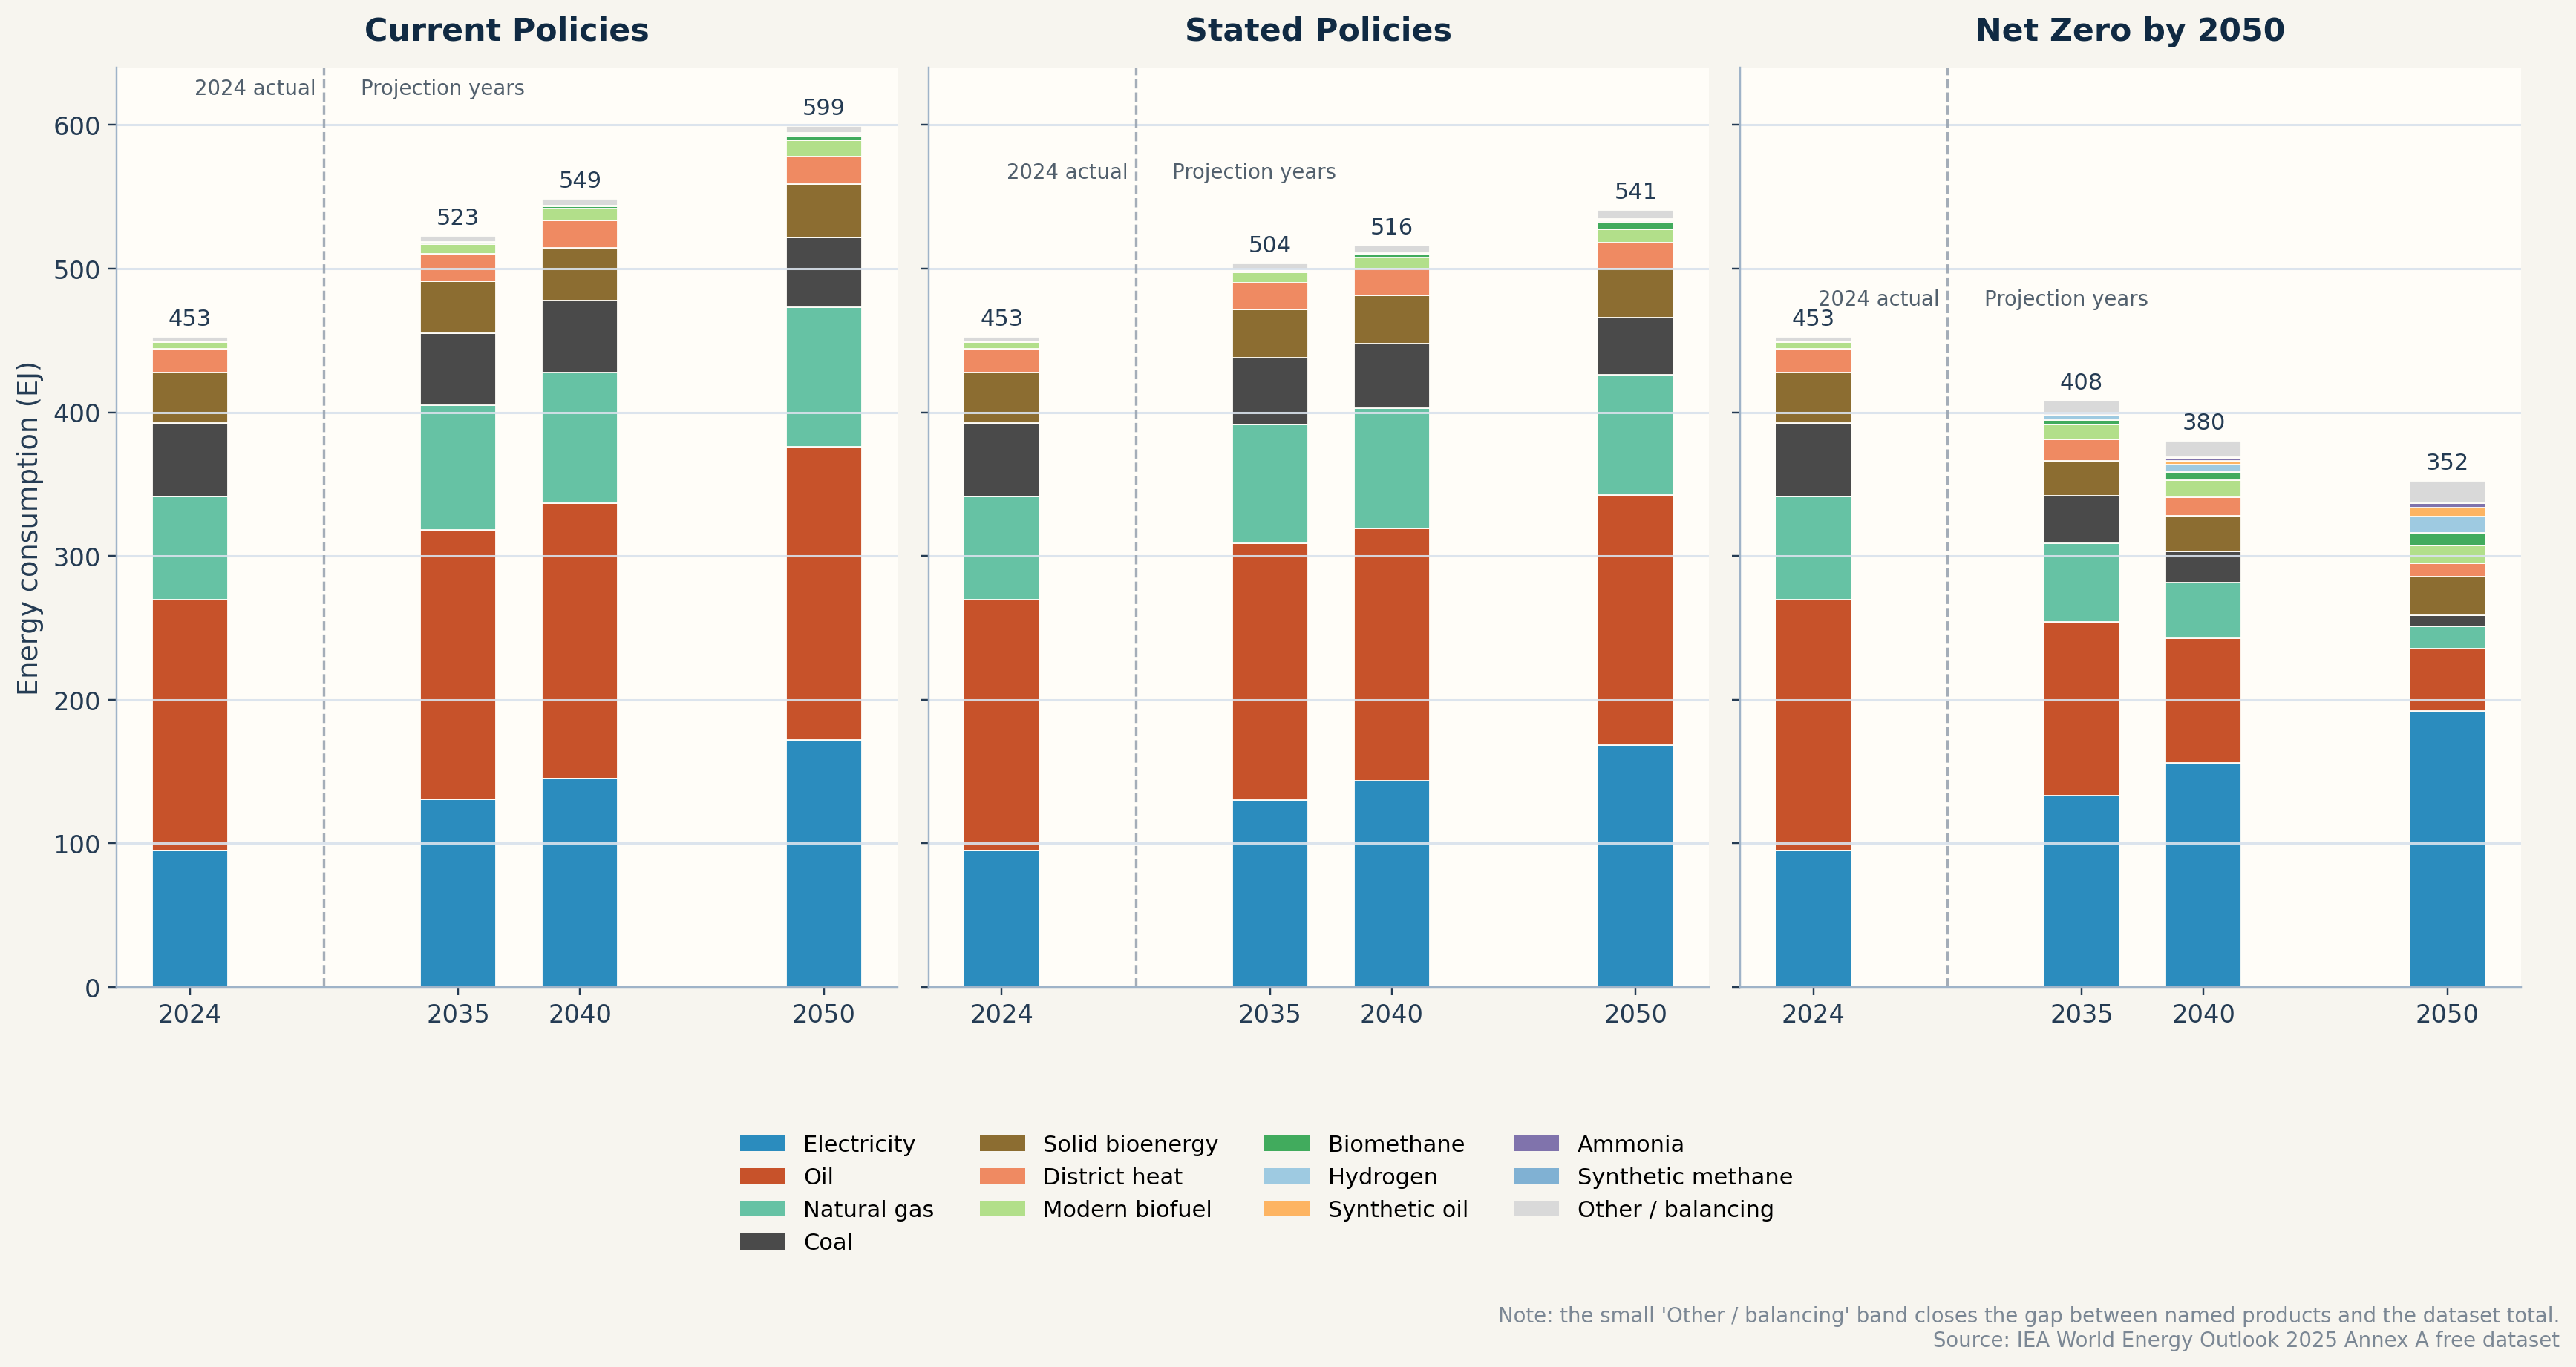
\includegraphics[width=\linewidth]{figures/world_energy_consumption_by_source_2050.png}
    \caption{World final energy consumption by source under the Current Policies, Stated Policies, and Net Zero Emissions by 2050 scenarios in the IEA World Energy Outlook 2025 free dataset.}
    \label{fig:world-energy-consumption-scenarios}
\end{figure}
 As shown in \Cref{fig:world-energy-consumption-scenarios}, global total final energy consumption rises from about 453~EJ in 2024 to roughly 599~EJ in 2050 in the Current Policies Scenario (CPS), where no strengthening of energy policies beyond those already in place is assumed. In the Stated Policies Scenario (STEPS), which incorporates a broader set of adopted and announced policy directions, demand still increases but more moderately, reaching about 541~EJ by 2050. By contrast, in the Net Zero Emissions by 2050 (NZE) Scenario, global final energy consumption falls to around 352~EJ by 2050, reflecting much stronger efficiency gains and a faster shift toward electrified end uses.

\begin{figure}[ht]
    \centering
    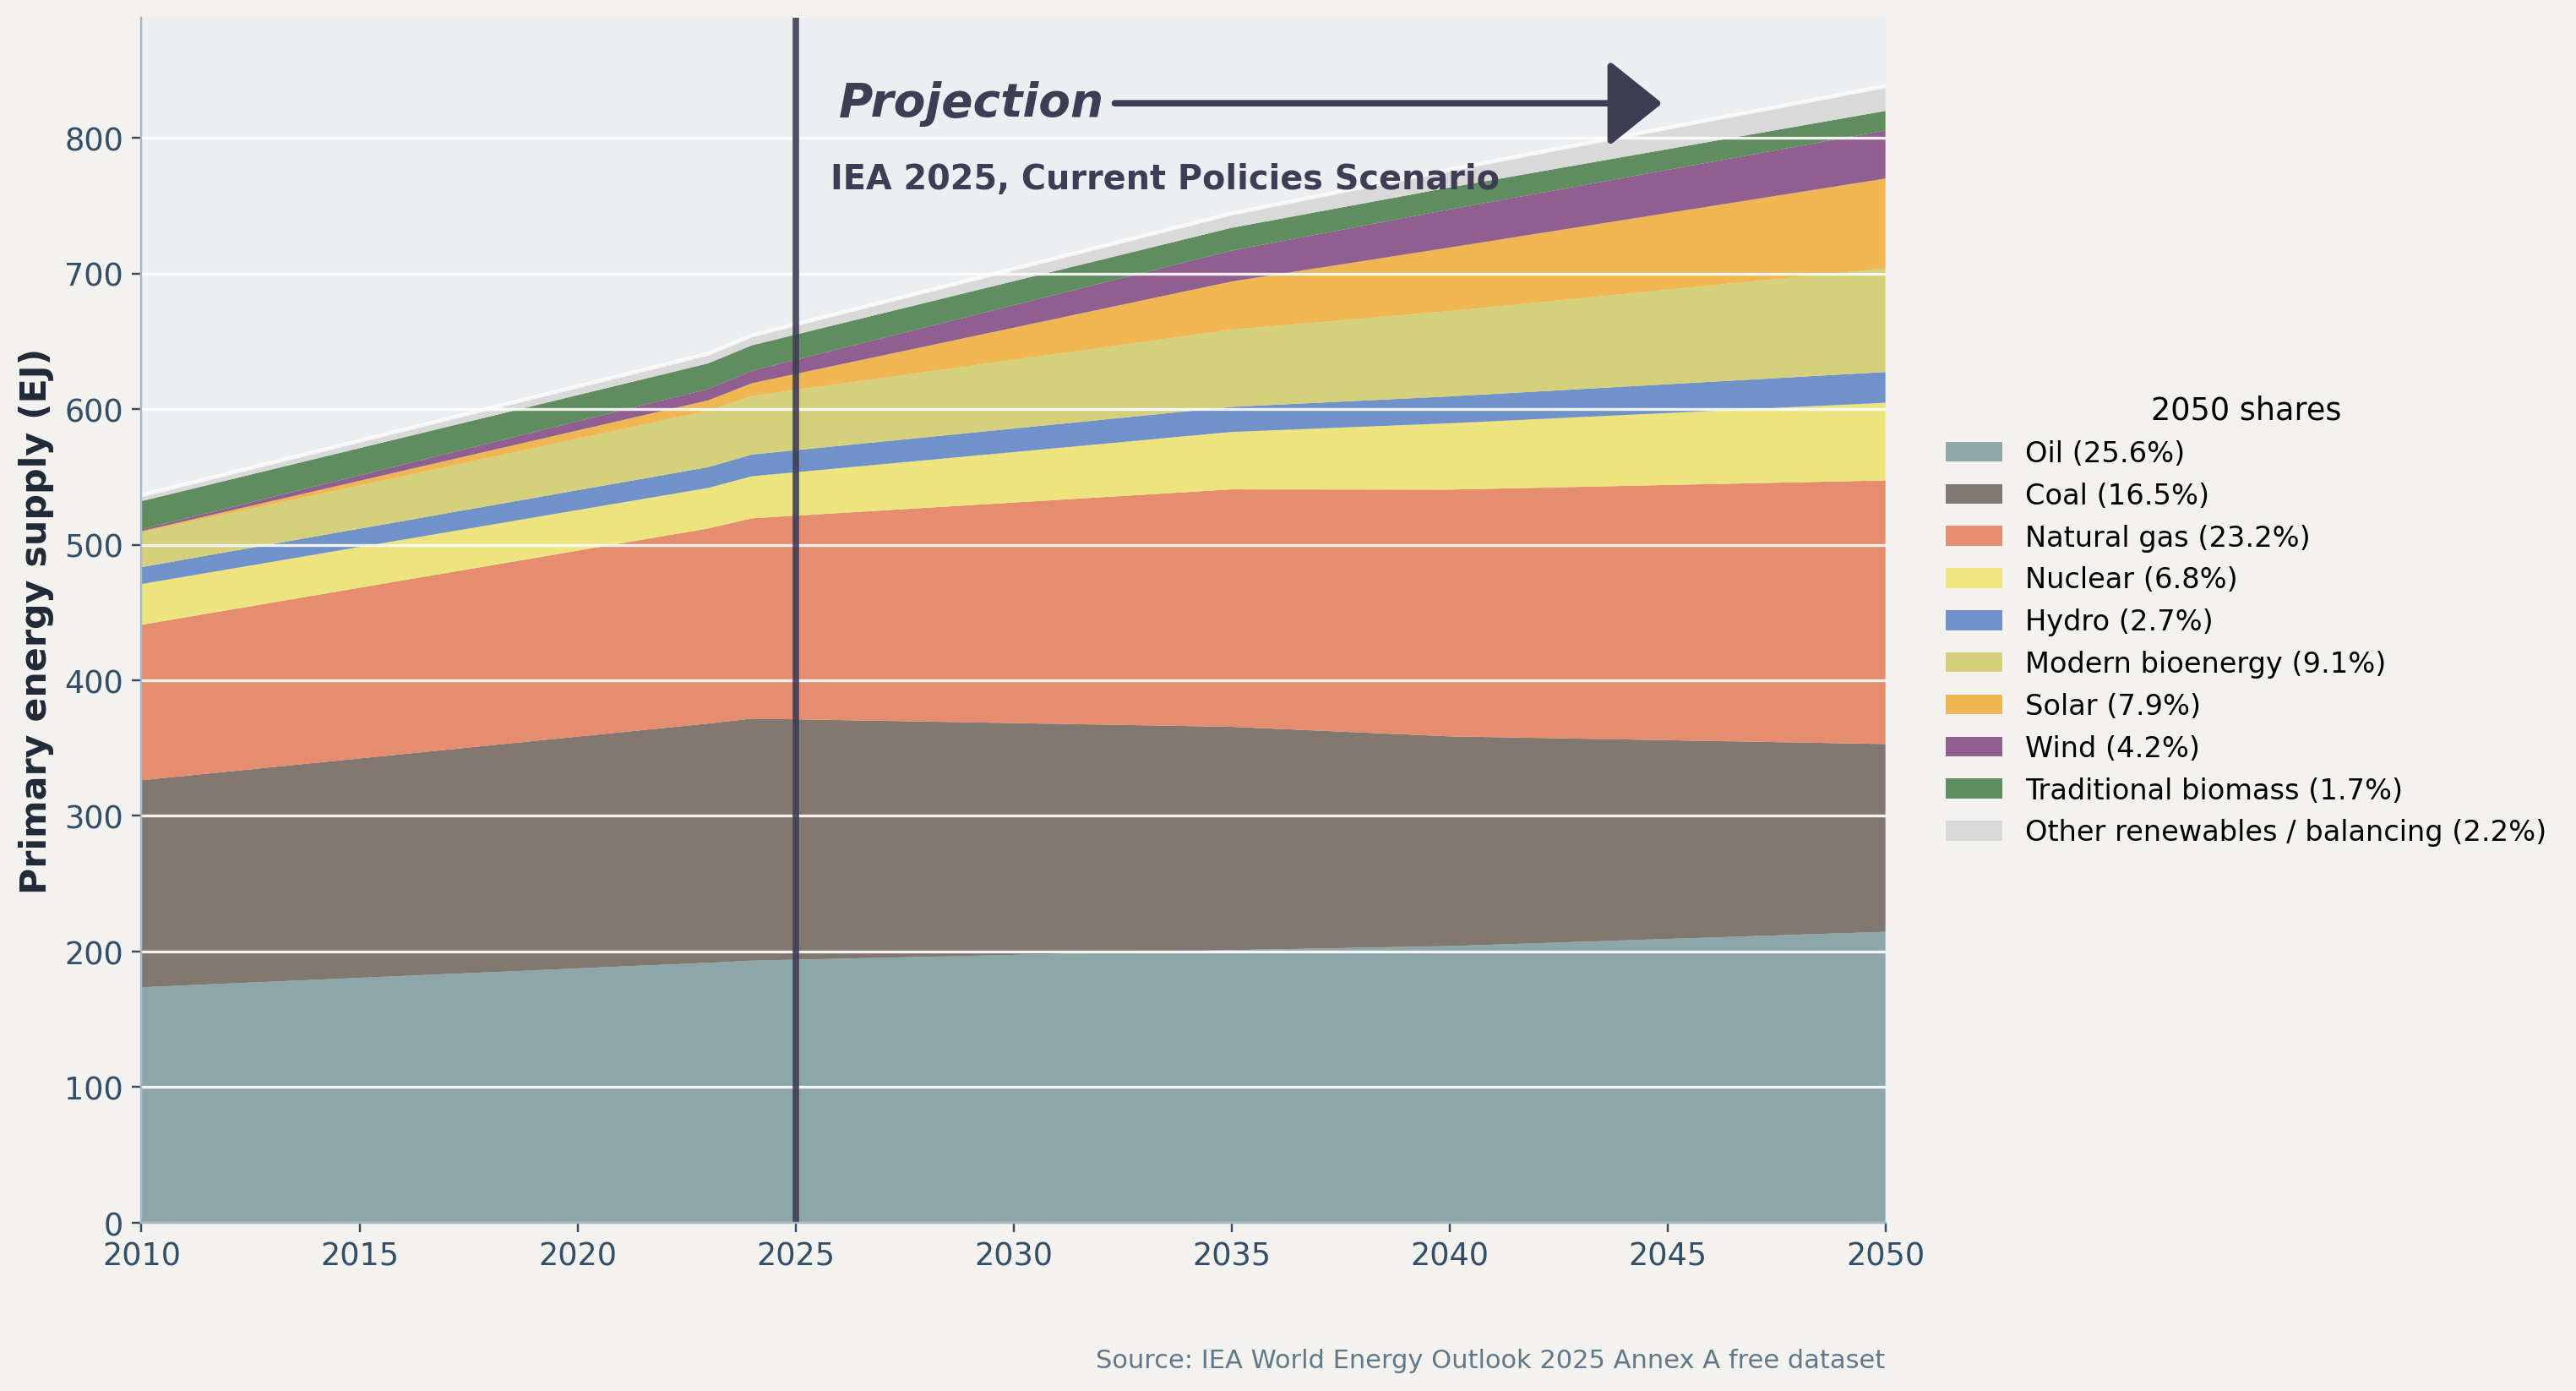
\includegraphics[width=\linewidth]{figures/world_energy_current_policies_shares_2050.png}
    \caption{World primary energy supply under the IEA World Energy Outlook 2025 Current Policies Scenario, with 2050 source shares shown in the legend.}
    \label{fig:world-current-policies-supply}
\end{figure}

\Cref{fig:world-current-policies-supply} complements this comparison by isolating the CPS pathway for world primary energy supply. Even in 2050, oil and natural gas remain the largest contributors, while solar, wind, nuclear, and modern bioenergy expand their shares substantially. This underlines why energy demand modelling is critical: future demand cannot be treated as a simple extrapolation of historical consumption, because it changes with assumptions about policy implementation, technology diffusion, fuel substitution, and energy efficiency. Scenario-based demand modelling is therefore essential for estimating future infrastructure needs, investment requirements, and emissions trajectories under different development pathways \cite{iea2025weo,iea2025gec}. 

\subsection{Technological Imperatives}
Inaccurate demand estimates can cause supply shortages or overcapacity, both of which drive price volatility and economic disruption. Geopolitically, detailed demand assessments also reveal import dependencies and exposure to external supply risks, informing diversification strategies and long-term energy-security policy.
\newline Beyond these considerations, there are fundamental technical reasons to map energy demand systematically, particularly in electricity. Power systems require real-time balancing: electricity must be consumed the instant it is generated \cite{WhyDoesElectricity}. If demand exceeds supply, system frequency drops and blackouts may follow; persistent overgeneration instead stresses system components \cite{ElectricalOvervoltageWhat}.

\subsubsection*{Grid frequency}
Frequency stability is thus a central operational constraint. In conventional systems dominated by large synchronous generators, the rotating masses of turbines and generators provide inertia. This does not eliminate imbalances but slows the rate at which frequency changes after a disturbance, buying time for control actions: after a sudden generation loss, inertia initially resists the frequency drop, after which primary frequency control, reserves, and other balancing services restore equilibrium. A lower-inertia system experiences a faster rate of change of frequency (RoCoF), leaving operators less time to respond and raising the risk of instability. Accurate demand modelling is therefore essential not only for energy accounting but for secure real-time operation, supporting reserve sizing, unit commitment, congestion management, and the anticipation of steep ramps and peak loads \cite{denholmInertiaPowerGrid2020}.

\subsubsection*{Infrastructure planning}
Demand mapping is equally critical for long-term infrastructure planning. Spatially resolved projections let policymakers and system operators anticipate urban growth, heating and transport electrification, and industrial development, informing timely investment in substations, transformers, transmission corridors, distribution reinforcements, and digital control infrastructure. Without sufficiently granular projections, network expansion can lag electrification, increasing congestion, curtailment, reliability risks, and total system cost \cite{entsoe_inertia_rocof_2020}.

\subsubsection*{Renewables}
The growing share of variable renewables such as wind and solar PV further raises the importance of detailed demand analysis. As noted in \Cref{sec:renewable_energy}, these resources are weather-dependent and only partially dispatchable, so their output need not coincide with peak demand. Many are also connected through power electronics rather than synchronous machines, so replacing thermal generation with inverter-based resources can reduce synchronous inertia, short-circuit strength, and the conventional frequency response naturally available, unless dedicated measures are introduced \cite{ElectricitySecurityMatters}. This again underscores the rising need for flexibility and coordination.

\subsection{Residential Energy Mix}\label{sec:residential_energy_mix}
A domestic (or residential) load is the energy a household uses to power all its appliances and devices, varying between households with their needs and consumption patterns.
\newline The residential sector is a significant source of energy-related GHG emissions, accounting for roughly 11\% of the global total once both direct fuel combustion and the indirect emissions from electricity and heat generation are included \cite{ritchieEmissionsBySector2020}. In 2023 it represented 26.2\% of EU final energy consumption \cite{EnergyConsumptionHouseholds}.
\newline Heating and cooling dominate household energy use in most countries. According to the IEA, the largest energy sources in Belgium's residential sector are natural gas and oil, at roughly 43\% and 27\% of residential final consumption respectively (\Cref{fig:BE_resi_consumption_mix}), with electricity (\textasciitilde20\%) and biofuels and waste (\textasciitilde9\%) making up most of the remainder \cite{IEA_ResidentialTFC_Belgium}. The sector is less well understood than commercial, industrial, agricultural, and transport demand, which benefit from more centralised ownership, stronger incentives and expertise in cutting consumption, and higher levels of regulation and documentation \cite{swan_modeling_2009}.
\begin{figure}[ht]
    \centering
    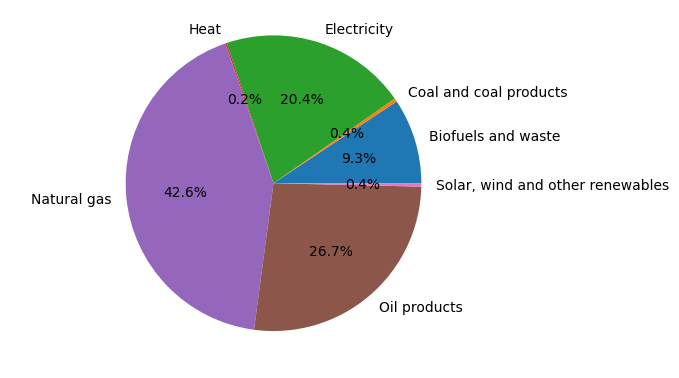
\includegraphics[width=0.8\linewidth]{figures/BE_resi_consumption.png}
    \caption{Belgian residential consumption mix in 2023; source: \href{https://www.iea.org/countries/belgium}{IEA}}
    \label{fig:BE_resi_consumption_mix}
\end{figure}
The residential sector consumes secondary energy: energy delivered ready for use to support occupants' living standards. Its main end-use groups are space heating and cooling (SH/SC), domestic hot water (DHW), and appliances and lighting. SH and SC offset thermal losses through the building envelope—conduction, radiation, and air infiltration/ventilation—to maintain a comfortable indoor temperature; DHW heats water for occupant and appliance use; and appliances and lighting power common devices (e.g.\ refrigerators, coffee makers) and provide adequate lighting. The relative weight of each group depends strongly on climate, building and system characteristics, appliance ownership, and occupant behaviour \cite{swan_modeling_2009}.

\subsubsection*{Electrifying the residential sector}
Many end uses in modern economies—lighting, information technology, household appliances, and air conditioning—are already electricity-based, but a large share of thermal demand is still met by directly combusting fuels: natural gas, heating oil, coal, and biomass remain widely used for space heating, DHW, and cooking. Electrifying these end uses is therefore a key mitigation pathway. Replacing fossil-fuel boilers with high-efficiency electric heat pumps can sharply reduce CO$_2$ emissions, especially as the electricity supply shifts toward low-carbon generation \cite{BelgiumCountriesRegions}, coupling end-use sectors to a progressively decarbonised power system.
\newline The transformation of the energy system should thus not be read as a trade-off between environmental and socio-economic objectives, but as a response to a single interconnected challenge. The same fossil-fuel combustion that drives environmental degradation also harms public health through air pollution, strains economies through climate-related damages, and undermines long-term societal stability. Decarbonising energy systems therefore advances environmental integrity, human well-being, and economic resilience together, since these dimensions are inherently interdependent.

\subsubsection*{New energy variables}
Historically, energy demand patterns exhibited relatively stable and predictable structures. Daily load curves largely reflected diurnal solar cycles\footnote{Diurnal solar cycles are the 24-hour patterns of change in sunlight, temperature, and atmospheric conditions driven by Earth's daily rotation. These cycles dictate the fluctuation between day and night, affecting energy input and causing daily temperature maximums in the afternoon and minimums at sunrise \cite{DiurnalCycle2025}.} and conventional work-week rhythms, with identifiable morning and evening peaks and reduced demand during nighttime and weekends. Under such conditions, forecasting approaches based primarily on historical time series and seasonal adjustments were often sufficient for operational planning.
\newline In contemporary energy systems, however, demand dynamics have become significantly more complex. Several structural developments contribute to this increased complexity:

\paragraph{Expansion of data centres.} 
Modern data centres require large amounts of continuous electricity, often operating as near-constant baseload consumers. Unlike residential loads, which fluctuate with occupancy patterns, data centre demand is relatively inelastic and geographically concentrated, placing sustained pressure on local grids.

\paragraph{Electrification of transport.} 
The rapid adoption of EVs introduces millions of distributed, mobile storage units into the electricity system. Charging behaviour is heterogeneous and time-dependent, often shifting demand from centralized workplace charging toward residential evening peaks. Without coordinated smart charging strategies, this can exacerbate peak loads and increase network congestion.

\paragraph{Climate variability.} 
Climate change introduces greater uncertainty into heating and cooling demand. Rising temperatures increase cooling loads, while more frequent and intense weather events reduce the reliability of historical data as a predictor of future energy consumption patterns. Traditional forecasting models calibrated on stationary climate assumptions may therefore become less accurate over time.

These developments fundamentally alter the temporal and spatial characteristics of energy demand. Consequently, accurate demand assessment can no longer rely solely on extrapolation of historical trends. Robust and physically grounded modelling frameworks are required to capture behavioural, technological, and climatic drivers of consumption. In this context, energy demand modelling emerges as a critical tool.


% \subsection{Residential Technologies}
% \label{sec:residentialTechnologies}
% % difference emitter vs conversion technologies
% % share of houses using PV, EV, heat pumps + boilers/gas in belgium

% \subsubsection*{Photovoltaics}
% %% 1-2 liner explanation on what PV is and how it works
% %% example of how it could be modelled, both simply and complex

% \subsubsection*{Electric vehicles}
% %% 1-2 liner explanation on what EV is and how it works
% %% example of how it could be modelled, both simply and complex

% \subsubsection*{Heat pumps}
% %% 1-2 liner explanation on what HP is and how it works: e.g.: 
% A heat pump (HP) uses mechanical work to pump heat from a low temperature to a high temperature. (the reverse of a heat pump is a refrigerant), using the vapor compression cycle.  The COP of a heat pump is a measure of its efficiency, calculated as the ratio of useful heat output (kW) to electrical power input (kW): $\text{COP}_\text{HP} = \frac{\dot{Q}_\text{H}}{\dot{W}_\text{in}}$ or $\text{COP}_\text{R} = \frac{\dot{Q}_\text{L}}{\dot{W}_\text{in}}$. However, this is an idealisation, referred to as the COP of Carnot, the ultimate efficiency that a heat pump can have. In reality, a pinch ($\Delta T)$ is necessary to drive the ``spontaneous'' heat transfer. Thus:
% \begin{align}
%     \text{COP}_\text{HP} &= \frac{\dot{Q}_\text{H}}{\dot{W}_\text{in}} = \frac{T_\text{H} + \Delta T}{T_\text{H} - T_\text{L} + 2\Delta T}\\
%     \text{COP}_\text{R} &= \frac{\dot{Q}_\text{L}}{\dot{W}_\text{in}} = \frac{T_\text{L} - \Delta T}{T_\text{H} - T_\text{L} + 2\Delta T}
% \end{align}
% %% example of how it could be modelled, both simply and complex, using HP implementation document (perhaps)?
% \paragraph{air-air HP}
% \paragraph{water-air HP}
% \paragraph{water-water HP}
% \paragraph{ground-source HP}

% \subsubsection*{Emitters}

\subsection{Residential Technologies}
\label{sec:residentialTechnologies}

Residential energy demand depends not only on the building envelope but on the technologies that convert energy carriers into useful services. These split usefully into \textit{conversion} technologies—which turn a carrier into heat, electricity, or mobility (gas boilers, heat pumps, PV systems, electric vehicles)—and \textit{emitter} technologies, which instead shape the conversion device's operating conditions. Radiators, underfloor heating, and fan coils, for instance, set the supply temperature a heating system must deliver and thus strongly affect heat-pump performance.

\subsubsection*{Belgian residential technology Stock}
Belgium's residential stock remains heavily fossil-based for space heating. The JRC reports roughly 2.8 million households using gas boilers against an installed heat-pump stock of about 209,000 units in 2022, when heat pumps made up only 11.8\% of combined heat-pump and boiler sales \cite{JRC2022HeatPumpBelgium}. Electrified technologies are nonetheless gaining ground: cumulative PV capacity reached 11.7\,GW in 2024, still dominated by sub-10\,kW residential systems \cite{vermang2024_pvps_belgium}. The same trend appears in transport, where households averaged 1.06 cars in 2024 \cite{StatbelHouseholds2025} amid a steadily hybridising and electrifying passenger fleet \cite{Statbel2025EV}. Such technologies are key boundary conditions for residential demand modelling, as they reshape both the annual energy balance and the timing of electricity demand.

\subsubsection*{Photovoltaics}

PV systems convert incident solar irradiance into direct-current electricity through the photovoltaic effect, after which an inverter converts the generated power to alternating current for household use or grid export. In residential applications, PV mainly acts as an on-site electricity-generation technology that reduces net grid import during sunny periods and can increase local self-consumption when combined with flexible demand, batteries, heat pumps or electric-vehicle charging.
\newline A simple PV model can represent generation as a linear function of plane-of-array irradiance and installed peak capacity:
\begin{equation}
    P_\text{PV}(t) = \eta_\text{PV} A_\text{PV} G_\text{POA}(t),
\end{equation}
where $\eta_\text{PV}$ is the module efficiency, $A_\text{PV}$ is the active module area and $G_\text{POA}$ is the plane-of-array irradiance. Equivalently, the system can be represented through a specific yield or capacity-factor profile multiplied by installed capacity. More detailed models add module temperature, inverter efficiency, orientation, tilt, shading, soiling and degradation effects \cite{duffie2013_solar_engineering,desoto2006_solar_model}. 
\newline For residential stock modelling, the appropriate level of detail depends on whether PV is used only as an annual energy contribution or whether the interaction with hourly household demand and self-consumption is analysed.

\subsubsection*{Electric vehicles}
An EV stores electrical energy in a battery and converts it into mechanical work through an electric drivetrain. For residential energy modelling, the vehicle itself is less important than its charging behaviour: arrival time, departure time, charger power, required trip energy, state of charge and user flexibility determine how mobility demand appears as household electricity demand.
\newline A simple EV model can assign a fixed daily charging energy to households with an EV and distribute it over an evening charging window:
\begin{equation}
    E_\text{EV,day} = e_\text{km} d_\text{day},
\end{equation}
where $e_\text{km}$ is the specific electricity consumption per kilometre and $d_\text{day}$ is the daily driven distance. A more detailed model could sample trips, arrival times, plug-in probability, charging power, battery capacity and state-of-charge (SoC) constraints, so that the charging load becomes an event-based process rather than a fixed profile \cite{richardson2013_ev_demand,muratori2018_ev_charging}. This distinction matters because uncontrolled EV charging can amplify evening peaks, while delayed or smart charging can shift demand toward periods of PV production or lower system load.

\subsubsection*{Heat pumps}
A heat pump (HP) uses mechanical or electrical work to move heat from a lower-temperature \textit{source} to a higher-temperature \textit{sink}. In heating mode, useful heat is delivered to the dwelling; in cooling mode, heat is removed from the conditioned space. The ideal heat-pump coefficient of performance is bounded by the Carnot limit:
\begin{equation}
    \text{COP}_{\text{HP,Carnot}}
    =
    \frac{T_\text{H}}{T_\text{H}-T_\text{L}},
\end{equation}
where $T_\text{H}$ and $T_\text{L}$ are absolute sink and source temperatures. For refrigeration or cooling, the corresponding ideal coefficient is:
\begin{equation}
    \text{COP}_{\text{R,Carnot}}
    =
    \frac{T_\text{L}}{T_\text{H}-T_\text{L}}.
\end{equation}
In practice, finite temperature differences are required in the evaporator and condenser to drive heat transfer. If a simplified temperature approach $\Delta T$ is introduced, the effective evaporating temperature is lower than the source temperature and the condensing temperature is higher than the sink temperature:
\begin{align}
    \text{COP}_\text{HP}
    &\approx
    \frac{T_\text{H} + \Delta T}
    {T_\text{H} - T_\text{L} + 2\Delta T}, \\
    \text{COP}_\text{R}
    &\approx
    \frac{T_\text{L} - \Delta T}
    {T_\text{H} - T_\text{L} + 2\Delta T}.
\end{align}
These expressions remain idealised, but they show the central physical dependency: heat pumps perform better when the temperature lift between source and sink is small~\cite{moran2018_thermodynamics,staffell2012_review_heat_pumps}.
\newline A simple heat-pump model can use a fixed seasonal performance factor (SPF) or constant COP:
\begin{equation}
    P_\text{el,HP}(t) =
    \frac{\dot{Q}_\text{useful}(t)}{\text{COP}}.
\end{equation}
This is sufficient for coarse annual energy balances, but it hides the dependence on outdoor temperature and supply temperature. More detailed models calculate COP as a function of source temperature, sink temperature, part-load operation, defrost losses\footnote{Defrost is the process where an air-source heat pump removes ice/frost from its outdoor coil. The frost comes from the moisture of the cold and humid air that freezes on the coil. That frost blocks airflow and reduces heat transfer, so the heat pump becomes less efficient.} and emitter type. This is particularly relevant in Belgian dwellings, where existing buildings often require higher supply temperatures than new low-temperature heating systems.

\paragraph{Air-air heat pumps.}
An air-air heat pump extracts heat from outdoor air and supplies heat directly to indoor air. It usually has relatively low distribution losses and can also provide active cooling, but it does not directly feed a hydronic radiator or DHW system. In residential models, it can be represented as an electricity-driven space-conditioning unit with outdoor-air temperature as the source and indoor air as the sink.

\paragraph{Air-water heat pumps.}
An air-water heat pump extracts heat from outdoor air and delivers heat to a water-based distribution system. This is one of the most relevant heat-pump types for residential space heating because it can replace or supplement boiler-based hydronic systems. Its performance is strongly affected by the required water supply temperature: underfloor heating and low-temperature radiators generally allow higher COPs than standard or high-temperature radiators.

\paragraph{Water-water heat pumps.}
A water-water heat pump uses water as the heat source and water as the heat sink. The source can be groundwater, surface water or another water loop. Since water-source temperatures are often more stable than outdoor air temperatures, water-water systems can achieve high and stable COPs. However, they are more site-specific and depend on hydraulic, environmental and regulatory constraints.

\paragraph{Ground-source heat pumps.}
A ground-source heat pump extracts heat from the ground through horizontal loops, vertical boreholes or brine circuits. The ground source is less variable than outdoor air, which reduces seasonal COP variation and avoids most defrost-related losses. The drawback is the higher installation complexity and cost, especially in dense residential areas or existing buildings.

\subsubsection*{Emitters}
Emitter systems transfer useful heat from the conversion technology to the indoor zone; common residential types are standard radiators, low-temperature radiators, underfloor heating, and fan coils. Their relevance to energy modelling lies in their required supply temperature. A gas boiler can deliver high supply temperatures with little efficiency penalty, whereas a heat pump loses efficiency as the sink temperature rises. The same heat pump can therefore draw different amounts of electricity depending on whether it serves underfloor heating, low-temperature radiators, or older high-temperature radiators.
\newline Simplified stock models can represent emitters through a fixed design supply temperature per dwelling class. A more detailed option is weather-compensated control, where the flow temperature tracks outdoor temperature rather than staying at the design maximum all season \cite{home_energy_model_heat_pumps_2026}:
\begin{equation}
    T_\text{supply}(t)
    =
    T_\text{low}
    +
    f(T_\text{out}(t))
    \left(
    T_\text{high} - T_\text{low}
    \right).
\end{equation}
This captures the link between building heat demand, outdoor conditions, emitter type, and heat-pump COP without a full hydraulic simulation. In technology scenarios, emitter assumptions thus decide whether heat-pump electrification is modelled as a low-temperature, high-COP pathway or a higher-temperature retrofit with lower seasonal performance.


\pagebreak
\section{Energy Demand Modelling}

Energy demand modelling can be defined as the quantitative determination of present and future energy consumption patterns through mathematical and computational models. These models are used to represent the structural drivers of demand and to project both long-term trends and short-term fluctuations. In doing so, they support system planning, sustainability assessment, and infrastructure optimization \cite{verwiebe_modeling_2021}. Depending on the modelling paradigm\footnote{A model's paradigm refers to the fundamental approach used to construct it.} adopted, demand models may range from high-level econometric representations to detailed, \hyperref[sec:bottom_up]{bottom-up} simulations of individual buildings and technologies. 
\newline \Cref{fig:modelling_framework} shows a \hyperref[sec:bottomUpModelling]{bottom-up modelling} framework adopted by Cruz et al.'s modelling paradigm.

\begin{figure}[ht]
    \centering
    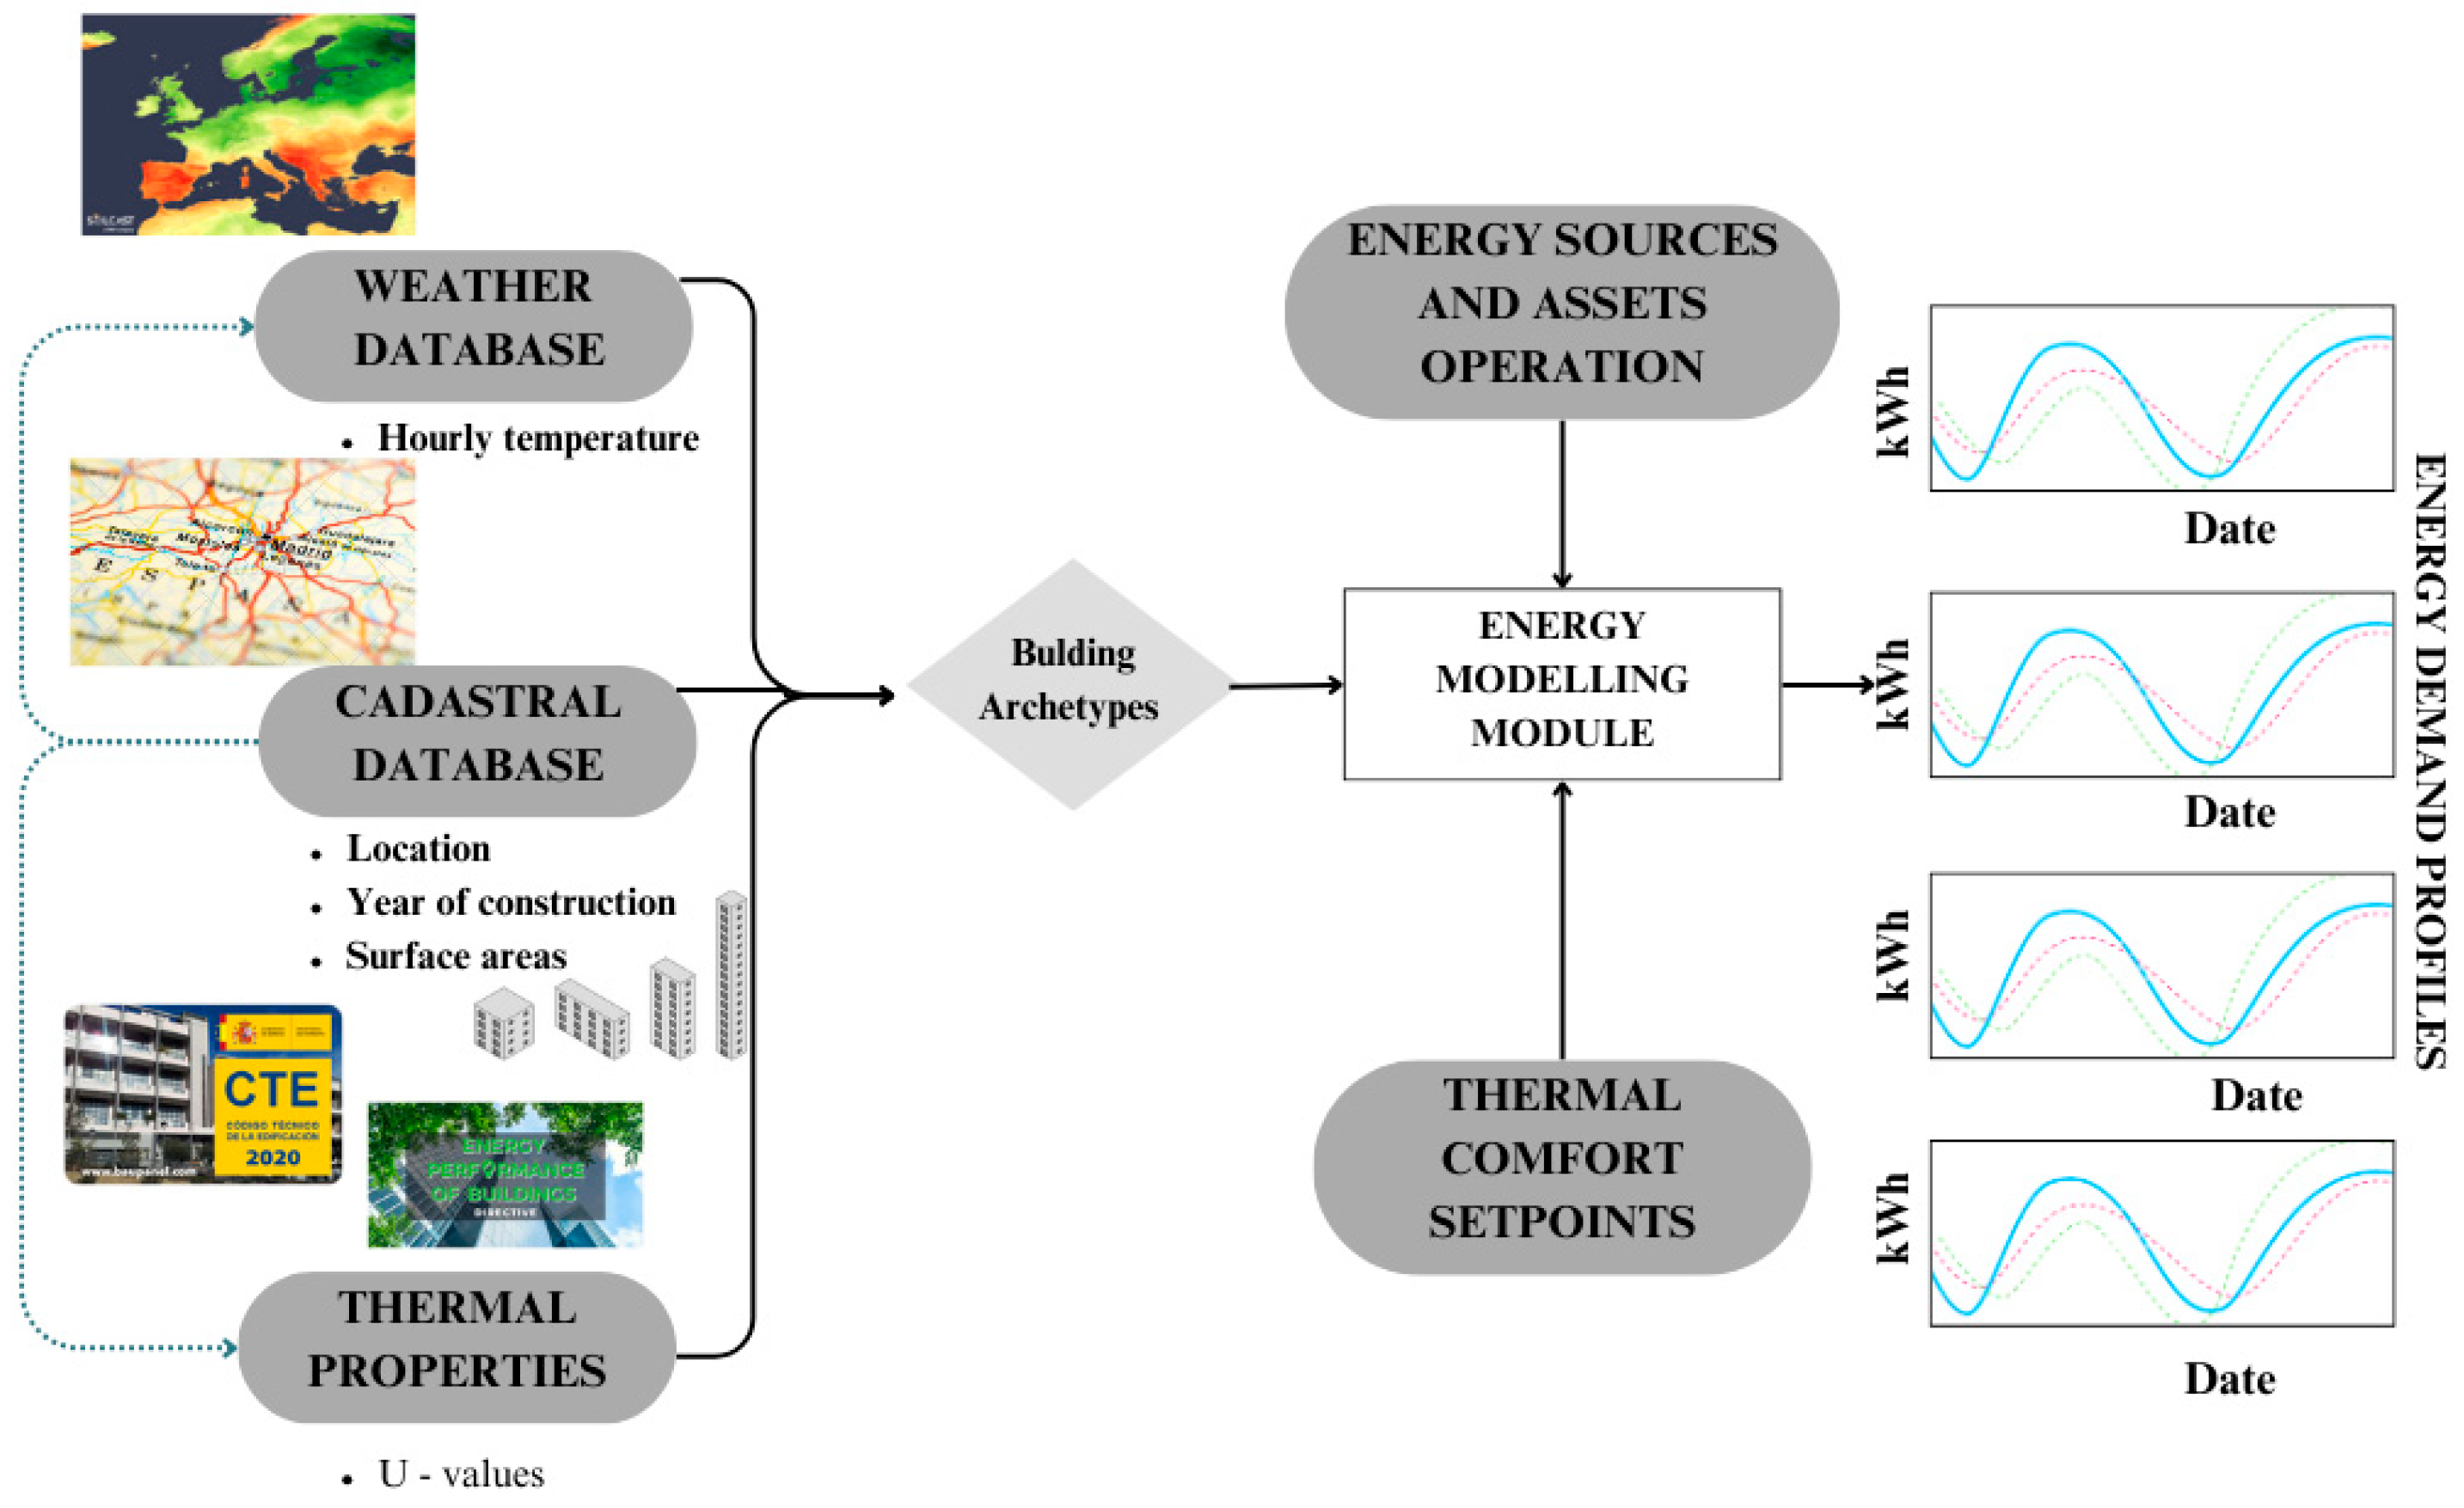
\includegraphics[width=0.8\linewidth]{figures/modelling_framework.png}
    \caption{Energy consumption modelling framework; source: Cruz et al.\cite{cruzDevelopmentEnergyDemand2025}}
    \label{fig:modelling_framework}
\end{figure}

Energy demand models are applied across multiple spatial and temporal scales. At the macro scale, they are commonly used to estimate regional, national, or supranational energy requirements and to inform long-term capacity expansion planning. At the micro scale, models can quantify the change in energy consumption of a specific dwelling\footnote{A dwelling is a home—see \Cref{sec:residential_eED_modelling} for a more detailed explanation.} due to technological upgrades, retrofits, or behavioural shifts. Such analyses are particularly relevant in the residential sector, where improvements in insulation, heating systems, glazing, or control strategies can significantly alter consumption profiles. By estimating both baseline demand and potential savings, these models provide quantitative support for policy decisions related to building codes, retrofit incentives\footnote{Retrofit incentives are financial or regulatory measures designed to encourage the upgrade of existing buildings or systems to improve their performance, typically in terms of energy efficiency or emissions reduction.}, electrification strategies, and long-term infrastructure investment \cite{swan_modeling_2009}.

% Models may be used for a variety of reasons, the most common being the determination of regional or national energy supply (macro-scale) requirements and the change in energy consumption of a particular dwelling\footnote{A dwelling is a home — somewhere to live.} due to an upgrade or addition of technology (micro-scale). Modelling of this nature is useful as it can guide decisions of policy regarding the residential stock, both old and new. By quantifying the consumption and predicting the impact or savings due to retrofits and new materials and technology, decisions can be made to support energy supply, retrofit and technology incentives, new building code, or even demolition and re-construction \cite{swan_modeling_2009}.

\subsection{Modelling Challenges}
A persistent challenge in energy modelling is the representation of occupant behaviour—especially within \hyperref[sec:residential_eED_modelling]{residential energy modelling}. Traditional engineering models often assume deterministic usage patterns or standardized occupancy schedules. However, empirical evidence shows that occupant behaviour is dynamic, heterogeneous, and influenced by a complex interplay of internal and external factors. These include socio-demographic characteristics, cultural norms, economic incentives, comfort preferences, building design, and real-time environmental conditions \cite{delzendehImpactOccupantsBehaviours2017}. The stochastic and adaptive nature of occupant interactions with heating, cooling, ventilation, and appliance systems introduces substantial uncertainty into building energy predictions. Addressing this complexity requires a multidisciplinary approach that integrates perspectives from sociology, psychology, economics, and behavioural sciences alongside engineering and design. 
\newline Thus, understanding occupants’ motivations, decision-making processes, and interaction patterns with building systems is essential for improving the predictive accuracy of demand models. Incorporating behavioural variability into modelling frameworks enhances their \hyperref[sec:realism]{realism} and strengthens their relevance for policy design, demand-side management, and long-term decarbonization planning \cite{delzendehImpactOccupantsBehaviours2017}.


\subsection{Stock Models}
% what is a stock model, how does it fit in the energy demand model paradigm?
Although the two fields overlap significantly, energy \textit{stock} modelling and energy \textit{demand} modelling are not the same. While the former provides the structural parameters of buildings, the latter simulates the dynamic energy flows. Residential stock modelling describes the ``shell'' (what exists), while residential energy demand modelling describes the ``energy flow'' (what happens inside) \cite{mahmoudOpportunitiesLimitationsBuilding2020}.

\subsubsection*{Building stock models}
Building stock energy refers to the aggregate energy consumption of all buildings in a given area. In the EU the building sector is a major share of final energy use and GHG emissions, with roughly 75\% of buildings classified as poor energy performers \cite{nageliBestPracticeReporting2022}. Because buildings are long-lived assets, decarbonising the stock is a structural challenge, and EU policy accordingly emphasises large-scale renovation and efficiency strategies. Building stock models are the central tool here: they let policymakers simulate renovation pathways, assess cost-optimal retrofits, estimate emission reductions, and track progress toward 2050 climate neutrality \cite{EUBuildingStock}, quantifying through scenario analysis the stock-wide impact of insulation upgrades, heating electrification, or district-heating expansion.
\newline Such models represent an entire building population within a defined area (city, region, or country) as a structured ensemble of archetypes, rather than a single building. Each archetype is characterised by parameters such as building type, construction period and typology, heating, cooling and DHW systems, and envelope properties such as U-values\footnote{The U-value measures how effectively a building element resists heat transfer, in W/m²K, across all its layers \cite{yuUValuesBuildingEnvelopes2024}.}. Aggregating these archetypes and scaling them to statistical data yields estimates of total energy demand, emissions, and renovation impacts at system scale \cite{hongTenQuestionsBuilding2025}. Building stock modelling is closely related to residential energy demand modelling but operates at a more aggregated, policy-oriented level; this review therefore concentrates on demand-modelling methodologies rather than large-scale stock transition modelling.


\subsubsection*{Residential stock models}
Residential stock modelling focuses on representing the structural composition and long-term evolution of the housing sector. Its primary objective is to characterize the building fleet at an aggregated level. Such models aim to provide a structured description of the physical and technical attributes of dwellings across a defined region \cite{hongTenQuestionsBuilding2025}.
\newline Although the present literature review focuses on residential buildings—specifically dwellings—it does not primarily address residential stock modelling in the structural or policy-oriented sense described above. Instead, the emphasis lies on modelling residential energy consumption: that is, the dynamic and quantitative simulation of energy use within dwellings.


\subsubsection*{Comparing stock and demand}
Table \ref{tab:modelling_framework_comparison} compares the two aforementioned modelling frameworks. 

\begin{table}[ht]
\centering
\caption{Comparison between residential stock modelling and residential energy cemand modelling}
\label{tab:modelling_framework_comparison}
\begin{tabular}{p{3cm} p{5cm} p{5cm}}
\toprule
\textbf{Aspect} & \textbf{Stock Modelling} & \textbf{Energy Demand Modelling} \\
\midrule
Focus & What buildings exist? & energy consumption \\
Nature & Structural, static & Dynamic, temporal \\
Time resolution & Usually none or annual & Hourly or sub-hourly \\
Core variable & U-values, system type & kWh, load profiles \\
Uncertainty type & Structural uncertainty & Behavioural + climate + system \\
\bottomrule
\end{tabular}
\end{table}
From a modelling pipeline perspective; the relation between the two frameworks could possibly look like this:
$$ \text{Building Stock Model  →  Parameterisation  →  Energy Demand Model} $$


\subsection{Residential Energy Demand Modelling}\label{sec:residential_eED_modelling}
Residential energy demand modelling quantifies household energy consumption over time. While it often draws on ``stock data'' as input, its main concern is the physics of energy use and human behaviour within a given \textit{dwelling} \cite{zhangModelingManagingResidential2025}. It answers questions such as: what is a household's hourly electricity demand, the annual space-heating demand of detached houses, the load profile of a community, or the change in demand under electrification or climate warming?

A dwelling—detached or semi-detached house, terraced house, flat, studio, and so on—is defined by having its own living spaces and facilities (sleeping, cooking, sanitation) separate from other units. Summing each dwelling's consumption across an area (city or country) gives the regional or national residential energy consumption that is the focus of this thesis.

Such models rely on input data to calculate or simulate consumption. The level of detail of that data varies dramatically, leading to different modelling techniques that exploit the available information, each with distinct strengths, weaknesses, capability, and applicability \cite{swan_modeling_2009}.


\subsection{Modelling Approaches}\label{sec:modelling_approaches}
Techniques used to model residential energy consumption are generally classified into two principal categories: top-down and bottom-up approaches. The distinction refers to the hierarchical level at which modelling inputs are introduced relative to the housing sector as a whole \cite{swan_modeling_2009}.

\subsubsection*{Overview of the top-down approach}
Top-down models begin at the aggregated level. They use macro-scale data—such as total residential energy consumption, gross domestic product\footnote{GDP is the total monetary value of all final goods and services produced within a country's borders during a specified period and is the most common measure of a nation's economic size and health.} (GDP), energy prices, demographic indicators, or climatic variables—to statistically attribute energy use to sector-wide characteristics. These models are typically econometric or regression-based and are well suited for national-level forecasting and policy analysis. However, they offer limited resolution regarding individual building characteristics or behavioural dynamics. 

\subsubsection*{Overview of the bottom-up approach}\label{sec:bottom_up}
Bottom-up models start at the micro scale. They simulate the energy consumption of individual dwellings or representative building archetypes based on physical properties, system specifications, occupancy patterns, and usage behaviour. The results are then aggregated to represent regional or national demand. Bottom-up approaches provide higher granularity\footnote{Granularity refers to the detail—both spatial and temporal—of the data/model.} and are particularly useful for evaluating retrofit strategies, electrification scenarios, and technology adoption pathways, because unlike the top-down approach, the bottom-up approach does have the ability to explicitly address the effect of occupant behaviour—which is a very important factor to consider when modelling energy consumption.

\subsubsection*{Top-down vs Bottom-up}
% Show table with pros and cons per modelling approach, also explain how they differ in realism and add a table that compares the two
Table \ref{tab:model_comparison} illustrates a comparative summary of the top-down and bottom-up approaches. The table summarizes their main characteristics, advantages, limitations, and relative level of \hyperref[sec:realism]{realism}.

\begin{table}[ht]
\centering
\footnotesize
\setlength{\tabcolsep}{4pt}
\renewcommand{\arraystretch}{1.2}
\caption{Comparison of top-down and bottom-up residential energy demand modelling approaches (adapted from Swan and Ugursal \cite{swan_modeling_2009}).}
\label{tab:model_comparison}
\begin{tabular}{>{\raggedright\arraybackslash}p{0.12\linewidth}
                >{\raggedright\arraybackslash}p{0.26\linewidth}
                >{\raggedright\arraybackslash}p{0.24\linewidth}
                >{\raggedright\arraybackslash}p{0.26\linewidth}}
\hline
\textbf{Approach} & \textbf{Main features} & \textbf{Advantages} & \textbf{Limitations / realism} \\
\hline
\textbf{Top-down} &
Uses aggregated sector-level energy data with macroeconomic, demographic, and climatic indicators; based on historical correlations and econometric models. &
- Suitable for long-term national or regional projections \newline
- Low data requirements \newline
- Computationally efficient &
- Limited technological granularity \newline
- Minimal behavioural representation \newline
- Lower physical realism \\
\hline
\textbf{Bottom-up} &
Estimates demand at the level of individual dwellings or archetypes, then aggregates to regional/national scale. Includes: \newline
(i) statistical methods \newline
(ii) engineering methods &
- Captures end-use detail \newline
- Can incorporate occupant behaviour \newline
- Suits retrofit and technology-impact analysis \newline
- Higher spatial and temporal resolution &
- Data intensive \newline
- Higher computational demand \newline
- Behaviour often simplified unless explicitly modelled \newline
- Requires calibration to reduce performance gap \newline
- Higher realism (physical + behavioural potential) \\
\hline
\end{tabular}
\end{table}

In terms of realism, top-down models provide the lowest structural fidelity because they rely on aggregate historical relationships rather than explicit physical representation. Bottom-up statistical models improve realism by capturing end-use diversity and behavioural correlations derived from empirical data. Bottom-up engineering models offer the highest level of physical realism, as they explicitly simulate thermodynamic processes and building-system interactions. However, their overall realism remains constrained if occupant behaviour is not represented stochastically or dynamically.
\newline Consequently, the choice of modelling approach depends on the research objective, data availability, and required resolution.


\subsection{Realism}\label{sec:realism}
In the context of energy demand modelling, realism refers to the extent to which a model accurately represents the physical, technical, and behavioural processes that determine actual energy consumption. A realistic model should not only reproduce aggregated annual consumption, but also capture temporal variability, system interactions, and user-driven dynamics that occur in practice.

\subsubsection*{Influential factors}
The energy consumption of buildings is influenced by a wide range of interacting factors, as is shown in \Cref{fig:influencing_factors}. These include the thermodynamic \& physical properties of buildings envelope, construction quality and detailing, climatic conditions, the performance and maintenance of HVAC systems, and—critically—the behaviour and activities of occupants \cite{delzendehImpactOccupantsBehaviours2017}, which is highlighted in \Cref{fig:influencing_factors} to emphasise its importance. 
\newline During the design phase, building energy simulation tools are typically employed to predict future consumption based on architectural plans, material specifications, and standardized occupancy assumptions. However, numerous empirical studies have documented a significant discrepancy between predicted and measured energy consumption in operational buildings \cite{delzendehImpactOccupantsBehaviours2017}. This discrepancy is commonly referred to as the performance gap.

\begin{figure}[ht]
    \centering
    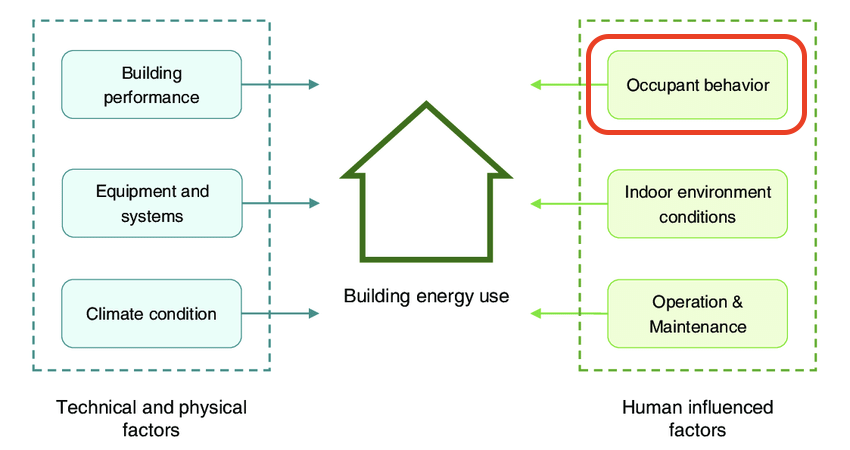
\includegraphics[width=0.8\linewidth]{figures/Six-influencing-factors-on-building-energy-use.png}
    \caption{Illustration of the six main influencing factors on a building's energy use; source: \href{https://www.researchgate.net/publication/337160052_China_Building_Energy_Use_2018}{China Building Energy Use 2018}}
    \label{fig:influencing_factors}
\end{figure}


\subsubsection*{Performance gap}
The performance gap arises from multiple sources. First, deviations between design intent and as-built construction—such as material substitutions, installation defects, or commissioning issues—can degrade performance. Second, operational conditions may differ from design assumptions. Most importantly, occupant behaviour is frequently simplified or treated deterministically in simulation tools. In reality, occupants exhibit heterogeneous, adaptive, and sometimes unpredictable behaviour patterns.

\subsubsection*{Occupant behaviour}
Research by Martinaitis and Zavadskas \cite{martinaitisImportanceOccupancyInformation2015} demonstrated that buildings often underperform relative to simulation results even when physical modelling is highly detailed, highlighting the decisive role of human behaviour. Similarly, Schakib-Ekbatan et al. \cite{schakib_ekbatanDoesOccupantBehavior2015} identified occupant behaviour as one of the most overlooked parameters in the entire chain of building design, construction, operation, and maintenance.
\newline Occupants influence energy use through variety of ways as displayed in \Cref{fig:behaviour_factors}. These behaviours are shaped by comfort preferences, socio-economic factors, cultural norms, and real-time environmental conditions. Because such behaviour is inherently dynamic with \hyperref[sec:stochastic_hetero]{stochasticity \& heterogeneity} at its core, deterministic schedules embedded in traditional simulation models often fail to capture realistic variability. As a result, improving the realism of building energy models increasingly requires explicit representation of occupant behaviour.

\begin{figure}[p]
    \centering
    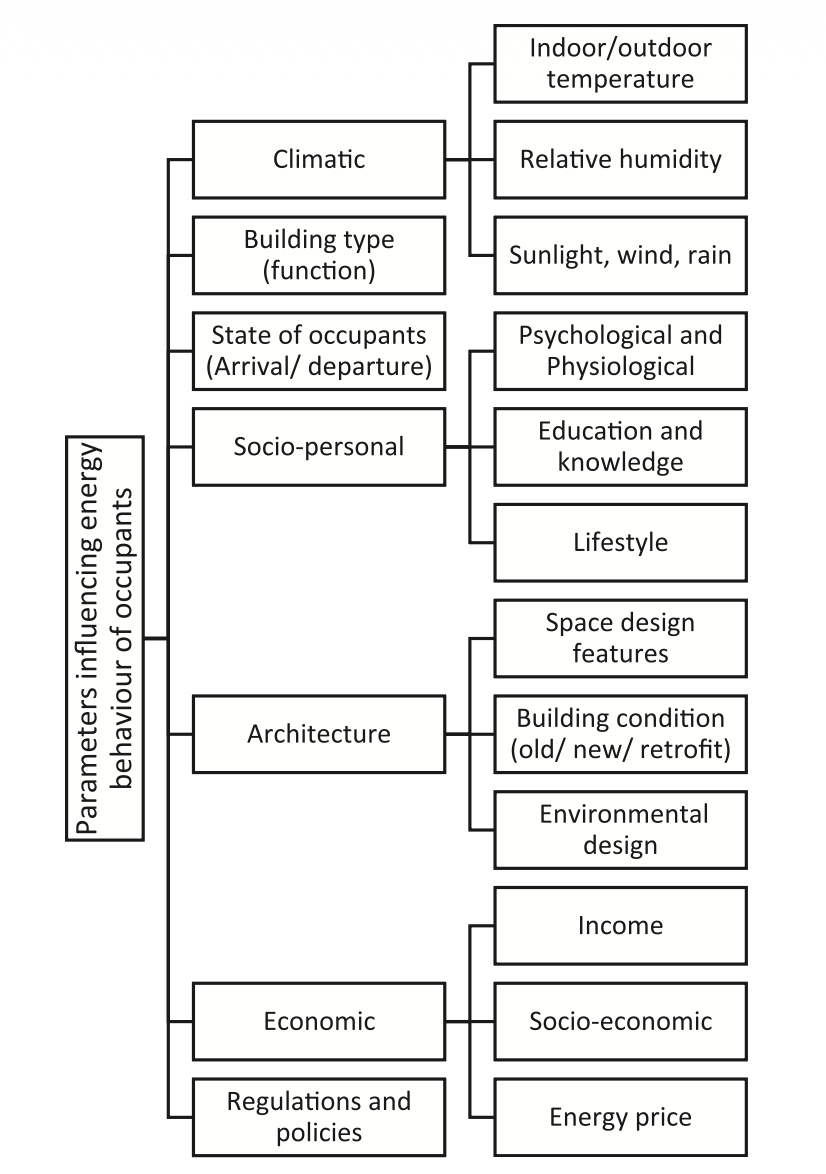
\includegraphics[width=0.8\linewidth]{figures/Behaviour_factors.png}
    \caption{Factors and sub-factors influencing energy behaviour of occupants \cite{delzendehImpactOccupantsBehaviours2017}.}
    \label{fig:behaviour_factors}
\end{figure}


\subsection{Uncertainty}
%%% what is uncertainty, how does it influence the models, what does the literature show, ...
The term ``uncertainty'' can be defined as the state of having limited knowledge about a system, making it difficult to predict future outcomes or describe current states accurately. A model which effectively captures different uncertainty sources has a higher degree of realism \cite{hongTenQuestionsBuilding2025,Smith2014}.

\subsubsection*{Sources of uncertainty}
One way to classify uncertainty sources is by distinguishing whether uncertainty is inherent to the system, due to lack of knowledge, or due to imperfect data \cite{Smith2014,Saltelli2008}.

\paragraph{Aleatoric uncertainty.}
This refers to the physical randomness of the system and is intrinsic — even with perfect knowledge, it does not disappear \cite{Smith2014}. In residential energy demand modelling, this is primarily associated with stochastic occupancy patterns and behavioural variability \cite{hongTenQuestionsBuilding2025}. This uncertainty is statistical in nature and must be modelled probabilistically.

\paragraph{Epistemic uncertainty.}
This arises from imperfect knowledge of the system or its parameters \cite{Smith2014}. In building energy models, this includes uncertainty in $U$-values, heat pump COP curves, thermal mass assumptions, and simplifications in model structure \cite{hongTenQuestionsBuilding2025,Hensen2011}. Unlike aleatoric uncertainty, epistemic uncertainty is reducible through improved data, calibration, and model refinement.

\paragraph{Data uncertainty.}
This refers to uncertainty introduced by imperfect, incomplete, or reconstructed data \cite{ASHRAE14}. Examples include missing weather data, smart meter gaps, temporal aggregation issues, and sensor noise. Such uncertainties propagate through the modelling pipeline and must be addressed prior to simulation.

To summarise, aleatoric uncertainty reflects inherent stochastic variability in occupant behaviour, epistemic uncertainty arises from incomplete knowledge of model parameters and structure, and data uncertainty originates from measurement errors and preprocessing steps, each requiring distinct modelling and validation strategies \cite{hongTenQuestionsBuilding2025,Smith2014}.


\subsection{Climate Uncertainty}
Climate conditions are a primary driver of residential energy demand, especially for space heating and cooling, which makes climate uncertainty a critical factor in energy modelling \cite{IPCC2021,DeWilde2014}. It arises from several sources: natural climate variability, structural differences between climate models, and uncertainty in future emissions scenarios \cite{IPCC2010}. In practice, this uncertainty enters through meteorological inputs such as outdoor temperature, solar irradiance, and wind speed. Temperature usually dominates thermal demand and is often approximated by aggregated indicators such as heating and cooling degree days (HDD/CDD) \cite{Clarke2001}. These are convenient but neglect temporal dynamics and non-linear system responses, which can bias demand estimates under changing climates \cite{DeWilde2014}.

A key distinction separates short-term variability, which drives demand fluctuations and peak loads, from long-term climate change, which shapes annual consumption and system sizing \cite{IPCC2021}. Representative weather datasets capture average conditions but miss extremes and inter-annual variability \cite{Wilcox2008}, so the literature increasingly favours multi-year datasets, stochastic weather generators, and climate-model ensembles to span a broader range of conditions \cite{Semenov2010,Saltelli2008}.
Integrating time-resolved weather variables directly into building energy models represents climate effects more consistently than aggregated indicators, which matters for non-linear processes such as thermal inertia, solar gains, and temperature-dependent system performance \cite{Clarke2001}. Explicitly accounting for climate uncertainty is therefore essential for robust, unbiased demand predictions under present and future climates \cite{DeWilde2014,IPCC2021}.


\subsection{Stochasticity \& Heterogeneity}\label{sec:stochastic_hetero}
In residential energy modelling, it is essential to distinguish between \textit{heterogeneity} and \textit{stochasticity}, as both concepts address different dimensions of aleatoric and epistemic uncertainty that drives a model's realism. 

Heterogeneity refers to systematic differences between households, whereas stochasticity refers to the time-varying and partly random behaviour within a given household. This distinction matters because empirical studies show that residential demand is neither well represented by a single “average household” nor by a deterministic repetition of the same daily routine. Instead, both the level of annual consumption and the timing of short-term demand events vary substantially across and within homes \cite{beis_ofgem_lv_network_capacity_2022}.

\subsubsection*{Heterogeneity}
Heterogeneity is clearest in the distribution of annual household demand: households do not consume uniformly. The differences stem from socio-demographic, technical, and environmental factors—occupant numbers, work and school schedules, lifestyle (e.g.\ cooking versus dining out), appliance ownership, and thermal-comfort expectations \cite{chen_stochastic_2022}.
\newline In a UK comparison of metered and simulated residential electricity data, Ramírez-Mendiola et al.\ \cite{ramirez_mendiola_grunewald_eyre_2017} find far greater dispersion in measured annual demand than in a widely used probabilistic simulation: across 243 households the coefficient of variation is 0.60 in the metered data versus 0.36 in the simulated, so the model under-represents cross-household diversity. The empirical distribution is also trimodal, with modes near 1.58, 3.92, and 7.85~MWh and mixture weights usable directly for calibration—evidence that inter-household variation is structured and multi-clustered rather than noise around one mean.
\newline This heterogeneity carries into peak demand relevant to network studies. Using smart-meter and demographic data from 2639 London households, Sun et al.\ \cite{sun_konstantelos_strbac_2016} show that diversified demand varies systematically with household composition and wealth: terminal After Diversity Maximum Demand\footnote{ADMD is an engineering estimate of the coincident maximum demand per customer, accounting for the fact that customers do not all peak simultaneously \cite{beis_ofgem_lv_network_capacity_2022}.} (ADMD) ranges from 0.51~kW for adverse one-occupant households to 1.72~kW for affluent households of three or more. Heterogeneity is thus measurable in the coincident peak that ultimately drives feeder and transformer loading, giving occupancy and socio-economic proxies direct engineering relevance.

\subsubsection*{Stochasticity}
Stochasticity concerns the irregular evolution of demand within a household or small group over time: even with fixed dwelling, appliances, and composition, use fluctuates because activities are not perfectly periodic. This variability is non-trivial. Anvari et al.\ \cite{anvari_et_al_2022} report that extreme consumption spikes vanish at 15-minute resolution because averaging smooths them out, yet these spikes matter precisely where low-voltage networks are stressed; their 15-minute diversity-factor analysis for 30 households reaches values of 0.6, showing that short-window coincidence stays substantial even at modest aggregation. Stochasticity therefore spans both random variation in appliance use, occupancy, and timing, and short-lived synchronisation effects invisible in coarse-resolution models.

\subsubsection*{Synchronisation risk}
The distinction matters most for synchronisation risk. A model that generates many households from one behavioural template, or reuses a single stochastic profile without structural variation, can artificially align demand peaks. UK network guidance from \href{https://www.spenergynetworks.co.uk}{SP Energy Networks} makes this concrete: in a cold-load-pickup condition after a significant winter outage, restored heat pumps all restart together and ``there is consequently no diversity'' \cite{spen_esdd_02_012_2024}. Coincident behaviour—physically real or accidentally imposed by the model—can thus produce materially higher aggregate peaks.

\subsubsection*{Diversified demand}
The need to represent heterogeneity is also clear from the non-linear scaling of diversified demand with household count. The UK Low Voltage Network Capacity Study reports large reductions from single-property to diversified feeder demand: depending on the DNO methodology\footnote{Distribution Network Operator (DNO) methodology is the operator-specific engineering approach used to estimate diversified demand \cite{beis_ofgem_lv_network_capacity_2022}.}, single-property values of 4.6--11.4~kW correspond to 120--211~kW for 100 homes, i.e.\ roughly 1.2--2.11~kW per dwelling after diversification \cite{beis_ofgem_lv_network_capacity_2022}. Coincident peak demand therefore does not scale linearly, and models that mishandle coincidence may over- or understate network requirements. Low-carbon dwellings point the same way: in a UK study of seven net-zero-ready homes with air-source heat pumps and PV, Millar et al.\ \cite{millar_weng_mateo_garcia_boyd_2025} measure diversified peak demand at just 14.6\% of total design capacity, with consumption largely occupancy-driven and heating and cooking exceeding 80\% of peak power. Installed capacity is thus a poor proxy for coincident demand, and occupancy-linked behaviour stays central even in highly electrified homes—so both heterogeneity and stochasticity remain critical under future low-carbon configurations.

\subsubsection*{Best representation}
Together, this literature shows that robust residential demand modelling requires explicit treatment of both heterogeneity and stochasticity: heterogeneity to reproduce the broad dispersion and clustering of peak-demand characteristics across households, and stochasticity to reproduce the irregular timing, short spikes, and intermittent coincidence within and across homes. A model capturing only one dimension will generally misrepresent aggregate residential load and may bias conclusions.


\subsection{Bottom-up Models}\label{sec:bottomUpModelling}
Bottom-up models are commonly divided into statistical and engineering (physics-based) approaches. Within the statistical branch, one can further distinguish between classical statistical models and data-driven / machine-learning models. \Cref{fig:bottom_up_hierarchy} displays a schematic overview of the relation between the bottom-up modelling approaches.  

\subsubsection*{Statistical methods}
% use the review papers to define and situate
A statistical method in bottom-up energy modelling estimates total residential energy consumption by analysing empirical data at the level of individual dwellings, households, or end-use components and subsequently aggregating the results. These approaches rely on historical billing data, surveys, or measured datasets to identify statistical relationships between energy use and its explanatory drivers (e.g., floor area, occupancy, appliance ownership, income, or climate variables) \cite{geraldiDatadrivenFrameworkRealistic2022}.
\newline An important strength of statistical bottom-up techniques is their ability to capture behavioural effects implicitly through observed data. Because occupant behaviour exhibits wide variability and is often poorly represented in deterministic engineering simulations, empirically derived correlations can provide valuable realism in residential modelling \cite{seryakOccupancyBehavioralAffects, emeryLongTermStudy2006}.
\newline Three well-documented statistical techniques \cite{swan_modeling_2009} are commonly applied:

\paragraph{Regression Analysis}
Regression-based models estimate energy consumption as a function of selected explanatory variables. Aggregate dwelling energy use is regressed against parameters expected to influence demand (e.g., building size, insulation level, occupancy, heating system type, or climatic indicators). Model performance is typically evaluated using goodness-of-fit metrics (e.g., $R^2$, RMSE). Variables with negligible explanatory power may be removed to simplify the model structure.
\newline Depending on the specification, regression coefficients may have limited or no direct physical interpretation. These models are particularly suitable when large datasets are available and when the objective is to identify statistically significant drivers of demand.

\paragraph{Conditional Demand Analysis}
Conditional Demand Analysis (CDA) estimates the contribution of individual end-uses by regressing total household energy consumption onto appliance ownership indicators. Appliances are typically represented as binary (present/absent) or count variables. The resulting regression coefficients approximate the average energy use associated with each appliance category.
\newline A big advantage of CDA is its relatively modest data requirement: appliance ownership surveys combined with utility billing data are often sufficient. The method exploits variation in appliance ownership across a large sample to infer end-use contributions. However, reliable estimation generally requires data from hundreds or thousands of dwellings to ensure sufficient statistical diversity and robustness.

\paragraph{Data-driven methods}
Within bottom-up modelling, data-driven models are generally situated under the statistical approach, since they infer energy-demand relationships directly from empirical observations rather than from explicit thermodynamic building equations. Machine-learning methods such as neural networks (NNs) therefore constitute a data-driven subset of statistical bottom-up models. 
\newline NNs are trained by minimizing prediction error, typically using gradient-based optimization. While they are capable of modelling nonlinear and highly interdependent relationships, the learned coefficients generally lack physical interpretability. As such, neural networks offer strong predictive performance but limited explanatory transparency.


\subsubsection*{Engineering methods}
Engineering methods—also called physics-based bottom-up models—estimate residential consumption by explicitly modelling the thermodynamic processes within buildings, typically applying building energy calculation procedures to a representative dwelling sample \cite{kavgicReviewBottomupBuilding2010}.
Unlike statistical approaches, they require detailed, physically measurable inputs: the thermal properties of envelope components, heating-system efficiencies and control characteristics, set-point temperatures and heating schedules, ventilation and infiltration rates, occupant numbers, and external climate data.
\newline Combining building physics with housing-survey data and operational assumptions, engineering models can estimate consumption for past, present, and future conditions, with scenario analysis enabling evaluation of retrofits, fuel switching, electrification, and carbon-reduction pathways \cite{kavgicReviewBottomupBuilding2010}.
\newline A key strength is independence from historical aggregate consumption data: being grounded in physical principles, these models can simulate technologies with no consumption record, such as high-efficiency heat pumps or advanced envelopes. Occupant behaviour, however, must usually be assumed rather than measured, and its wide variability introduces uncertainty that feeds the well-documented gap between predicted and measured consumption. Complexity ranges from simplified estimates based on heating degree days\footnote{HDD estimates heating energy demand from how many degrees the average daily outdoor temperature falls below a base temperature, typically around $18.3^{\circ}C$ \cite{usdepartmentofcommerceWhatAreHeating}.} (HDD) to detailed dynamic simulations of heat transfer, internal gains, and system control.
\newline Swan and Ugursal \cite{swan_modeling_2009} identify three principal engineering approaches:

\paragraph{Distribution-based models}
This technique combines statistical distributions of appliance ownership and usage with rated appliance power and efficiency values. Energy consumption is calculated separately for each end-use as:
$$ E= \text{Ownership} \times \text{Usage} \times \text{Rated Power} \times \mathrm{\frac{1}{Efficiency}}$$
Total residential demand is obtained by aggregating end-uses at regional or national scale. While computationally efficient, this method typically neglects interactions between end-uses (e.g., internal heat gains affecting heating demand).
\paragraph{Archetype models}
The housing stock is classified into representative archetypes based on characteristics such as construction period, dwelling type, size, or heating system. Each archetype is modelled using building physics methods, and results are scaled according to the number of dwellings belonging to each category. Archetype modelling offers a balance between computational tractability and physical detail, and is widely used in national building stock analyses.
\paragraph{Sample-based models}
This method uses detailed data from an actual sample of dwellings as direct model inputs. If the sample is statistically representative, results can be weighted and extrapolated to estimate regional or national energy consumption. Sample-based approaches capture greater diversity within the stock but require large, high-quality datasets.


%[also include data-driven modeling]
\subsubsection*{Hybrid models}
Although engineering models are grounded in thermodynamic principles, they inevitably rely on statistical inputs for several empirical parameters. For example, average DHW demand per person, appliance usage frequencies, internal heat gains, and occupancy schedules are often derived from survey data or monitored datasets \cite{kavgicReviewBottomupBuilding2010}. In this sense, purely physics-based modelling is rarely entirely independent of statistical assumptions.
\newline More advanced modelling frameworks therefore adopt a hybrid structure, integrating both building physics and statistical components in a systematic manner. In such models, heat transfer and system performance are computed using first-principles equations, while behavioural patterns, appliance usage, and stochastic occupancy dynamics are represented probabilistically or through empirically calibrated distributions. This integrated approach enhances realism by combining physical causality with empirically observed variability. Consequently, the distinction between statistical and engineering methods should not be interpreted as strictly binary.


\subsection{Conclusion}
Energy demand modelling spans approaches that differ in scale, realism, and data needs: top-down models give efficient aggregated projections but limited physical and behavioural resolution, whereas bottom-up models operate at the dwelling or archetype level and explicitly represent building characteristics and end uses. Within bottom-up frameworks, statistical methods capture empirical correlations from observed data while engineering models simulate thermodynamic processes and system performance, yet the literature consistently identifies occupant behaviour as a dominant source of uncertainty—making it essential to represent both heterogeneity between households and stochastic variability within them. Climate is an equally critical driver, since temperature and solar conditions govern heating and cooling demand; relying on aggregated indicators or single representative weather years understates extremes and inter-annual variability, so time-resolved weather and climate uncertainty must be handled explicitly. Robust residential demand modelling therefore requires an integrated approach combining physical building representation, behavioural variability, climate uncertainty, and appropriate temporal resolution to reliably reflect real-world consumption dynamics.

\begin{figure}[p]
\centering
\vspace*{\fill}
\resizebox{\textwidth}{!}{%
\begin{tikzpicture}[
    >=Latex,
    line/.style={draw, -Latex, line width=0.9pt},
    box/.style={
        draw,
        rounded corners=6pt,
        align=center,
        minimum height=11mm,
        inner sep=5pt,
        font=\large
    },
    smallbox/.style={
        draw,
        rounded corners=4pt,
        align=center,
        minimum height=9mm,
        inner sep=4pt,
        font=\normalsize
    }
]
% Top node
\node[box, minimum width=6.8cm] (top) at (0,0) {Bottom-up Models};
% Main branches
\node[box, minimum width=3.8cm] (stat) at (-6,-3.2) {Statistical};
\node[box, minimum width=4.2cm] (eng)  at ( 6,-3.2) {Engineering};
% Vertical trunks
\coordinate (split) at (0,-1.7);
\coordinate (statTop) at (-6,-1.7);
\coordinate (engTop)  at ( 6,-1.7);
% Statistical children
\node[smallbox, minimum width=3.4cm] (reg) at (-3.2,-6.0) {Regression};
\node[smallbox, minimum width=2.3cm] (cda) at (-3.8,-8.2) {CDA};
\node[smallbox, minimum width=2.3cm] (ml)  at (-3.8,-10.4) {ML};
% Engineering children
\node[smallbox, minimum width=3.5cm] (dist) at (3.2,-6.0) {Distribution};
\node[smallbox, minimum width=3.2cm] (arch) at (3.2,-8.2) {Archetype};
\node[smallbox, minimum width=3.4cm] (clust) at (3.2,-10.4) {Sample};
% Hybrid node
\node[box, minimum width=5.4cm] (hyb) at (0,-13.2) {Hybrid Models};
% Top connections
\draw[line] (top.south) -- (split);
\draw[line] (split) -| (stat.north);
\draw[line] (split) -| (eng.north);
% Statistical trunk and branches
\draw[line] (stat.south) -- ++(0,-8.7) coordinate (statBottom);
\draw[line] (-6,-6.0) -- (reg.west);
\draw[line] (-6,-8.2) -- (cda.west);
\draw[line] (-6,-10.4) -- (ml.west);
% Engineering trunk and branches
\draw[line] (eng.south) -- ++(0,-8.7) coordinate (engBottom);
\draw[line] (6,-6.0) -- (dist.east);
\draw[line] (6,-8.2) -- (arch.east);
\draw[line] (6,-10.4) -- (clust.east);
% Convergence to hybrid
\draw[line] (statBottom) |- (hyb.west);
\draw[line] (engBottom)  |- (hyb.east);
\end{tikzpicture}%
}
\vspace*{\fill}
\caption{Schematic overview of bottom-up modelling approaches.}
\label{fig:bottom_up_hierarchy}
\end{figure}


\pagebreak
% \section{Renewable Energy Communities}
% %  [needs more details, studies, results, situation in belgium...; but maybe wait with this section]
% % Define, map out, relate to residential energy demand modelling.
% Renewable Energy Communities (RECs) are legally recognized, democratically governed groups of local actors that collectively produce, consume, share and manage renewable energy for mutual environmental, economic and social benefit. Members may include households, small businesses, local authorities and other organizations. RECs aim to optimize local use of renewable energy, reduce reliance on fossil fuels, and provide services like demand flexibility and energy efficiency \cite{EnergyCommunity2026}.

% The following features can be assigned to RECs \cite{EnergyCommunity2026, corasanitiRenewableEnergyCommunities2025, EnergyCommunities}:
% \begin{itemize}
%     \item Open, voluntary participation: Members join by choice and share decision-making.
%     \item Local co-ownership and control: Members located near renewable generation assets have effective control.
%     \item Collective production and consumption: Members jointly produce, manage, and use renewable energy.
%     \item Environmental/economic benefits: RECs are structured to deliver local social or economic benefits (e.g., lower bills, local jobs). 
% \end{itemize}

% Corasaniti et al. \cite{corasanitiRenewableEnergyCommunities2025} describe RECs as “an innovative model for energy production, consumption, and sharing,” emphasizing decentralization and participation as defining aspects


% \subsection{Relationship with Residential Energy Demand}
% RECs intersect with residential demand in several fundamental ways \cite{ercoliDemandResponseRenewable2025, EnergyCommunities, corasanitiRenewableEnergyCommunities2025}. 

% \subsubsection*{Balancing load generation demand}
% Household electricity use often does not naturally align with renewable generation (e.g., PV output peaks midday while demand peaks at night). Effective REC operation requires detailed analysis of residential load profiles and strategies to adjust consumption patterns or storage use.
% \subsubsection*{Demand-side management}
% Demand flexibility techniques (e.g., shifting appliance use to times of high local generation) are central to REC performance. Ercoli et al. \cite{ercoliDemandResponseRenewable2025} show that coordinated demand response within a REC can meaningfully increase solar self-consumption and reduce community electricity costs.

% \subsubsection*{Residential load forecasting}
% Recent work uses machine learning to map hourly residential load profiles for REC planning and optimization, enabling better alignment between community supply and individual demand patterns.

% \subsubsection*{Residential self-consumption maximisation}
% Evaluated strategies \cite{hussainEnhancingRenewableEnergy2024} include:
% \begin{itemize}
%     \item Community storage shared across households to capture midday PV generation.
%     \item Internal energy trading among community members to increase local use of renewables.
% \end{itemize}


% \subsection{Residential Benefits}
% There are residential-level benefits tied to RECs \cite{ercoliDemandResponseRenewable2025, EnergyCommunities, corasanitiRenewableEnergyCommunities2025}:
% \begin{itemize}
%     \item Reduced electricity costs through localized pricing and self-consumption.
%     \item Enhanced energy autonomy for households, reducing dependence on distant generation.
%     \item Flexibility and demand management that can smooth peak loads and reduce grid stress.
%     \item Local economic and social benefits, including job creation and community engagement.
% \end{itemize}








% %%%%%%%% VERSION 1 %%%%%%%%

% % \section{Energy Demand}
% % The residential energy sector is undergoing rapid structural transformation driven by electrification and decarbonization. The deployment of electric heat pumps (HPs) as replacements for fossil-based heating systems and the accelerated adoption of electric vehicles (EVs) are fundamentally altering both the magnitude and temporal structure of the electricity demand. Unlike traditional household plug loads, these technologies introduce large, weather-dependent, and behaviour-sensitive electrical loads into the grid.

% % For example, air-to-water heat pumps exhibit strong performance variability between rated and in-use conditions, leading to discrepancies between expected and realized electricity consumption \cite{OHegarty2022_AWHPPerformanceGap, lammle_performance_2022}. Similarly, EV charging introduces high-power, temporally clustered loads that are driven by mobility behaviour rather than thermal demand dynamics (\cite{lekhel_generic_2025}). Therefore, the interaction between heating electrification and transport electrification creates new peak-load conditions, alters diversity factors, and increases system stress at the distribution levels.

% % This transformation implies that traditional aggregated load models are no longer sufficient. Electrified residential demand exhibits strong intra-day variability, coincidence effects, and stochastic user-dependent behaviour, necessitating bottom-up modelling approaches capable of resolving high-frequency dynamics.


% % \subsection{Renewable Energy Communities}

% % Renewable Energy Communities (RECs) introduce a new operational layer to residential demand modelling. In these systems, \textit{prosumers} collectively manage generation, storage, and demand to increase self-consumption and minimize grid interaction. Accurate forecasting becomes essential not merely for predictive accuracy, but for operational value.

% % Data-driven demand forecasting in RECs has shown that model quality does not necessarily translate directly into improved operational outcomes (\cite{coignard_evaluating_2021}). The timing of forecast errors can significantly affect battery dispatch, fairness allocation, and self-sufficiency metrics. Therefore, load modelling must consider not only deterministic prediction but uncertainty characterization.

% % In electrified communities, heat pumps, EVs, and distributed PV systems interact dynamically. The temporal coincidence between heating demand and low solar generation, or EV charging and evening peak load, creates system-level sensitivities. These interactions require modelling frameworks capable of propagating uncertainty from household behaviour to community-level performance.

% % \subsection{Importance of High-Resolution Demand Modelling}

% % High-resolution demand modelling is essential to capture diversity factors, switching behavior, and intra-hour variability. Classic bottom-up approaches have demonstrated that minute-level or sub-hourly resolution significantly improves realism compared to hourly aggregation (\cite{Richardson2010_DomesticHighRes, thorve_high_2023}).

% % Stochastic activity-based models translate occupant behavior into appliance activation patterns and resulting load profiles (\cite{Widén2009_StochasticActivity}). These approaches preserve diversity across dwellings and reduce artificial synchronization effects, which are common in deterministic scheduling models.

% % Similarly, stochastic bottom-up heating models capture variability in space heating and domestic hot water consumption, particularly under weather-driven conditions (\cite{Fischer2016_StochasticBottomUpHeatDHW}). High-resolution digital twin datasets further demonstrate the feasibility of generating large-scale disaggregated residential demand time series (\cite{thorve_high_2023}).

% % At city scale, two-step forecasting approaches combine building archetypes with statistical prediction layers to scale bottom-up modelling to urban contexts (\cite{yu_two-step_2018, frayssinet_modeling_2018}). However, these models often rely on deterministic building physics or averaged behavioral assumptions.


% % The increasing penetration of flexible electrified loads makes high-temporal resolution not optional but structurally necessary for capturing peak dynamics, rebound effects, and control opportunities.

% % \subsection{Deterministic Versus Stochastic Modelling Paradigms}

% % Traditional deterministic bottom-up models simulate appliance operation, heating loads, and occupancy schedules based on fixed or rule-based assumptions (\cite{Paatero2006_LoadProfileModel, subbiah_energy_2017}). While physically interpretable, such approaches risk underestimating variability and correlation structures inherent in real-world demand.

% % In contrast, stochastic models explicitly incorporate probabilistic representations of occupant behavior, appliance activation, and thermal response. Occupancy sequence generation methods produce realistic temporal patterns that better replicate empirical distributions (\cite{Aerts2017_RealisticOccupancySequences, rouleau_unified_2019}). Second-order thermal network models introduce dynamic thermal inertia effects that respond probabilistically to weather and control signals (\cite{wang_development_2022}).

% % Stochastic frameworks are particularly important under climate change and long-term electrification scenarios. Climate-induced shifts in heating and cooling demand require modelling approaches that integrate probabilistic weather inputs with building stock evolution (\cite{elnagar_modeling_2021}). Spatially explicit bottom-up stock models further highlight the importance of capturing heterogeneity at regional scale (\cite{dalonzo_bottom-up_2019}).

% % The paradigm shift from deterministic to stochastic modelling reflects a broader transition: from average load estimation toward uncertainty-aware energy system analysis. Electrified residential demand is no longer a static profile but a probabilistic process shaped by occupant behaviour, technology adoption, and climate variability.

% % In the context of RECs and grid-interactive buildings, modelling frameworks must therefore transition from deterministic schedule generation to fully stochastic, bottom-up representations capable of uncertainty propagation across scales.


% % \section{Modelling Paradigms in Residential Energy Demand}

% % \subsection{Top-Down Statistical Approaches}

% % Top-down modelling approaches represent residential energy demand at an aggregated level, typically at regional, national, or utility scale. These methods rely on historical consumption data and explanatory variables such as weather indicators, socio-economic factors, or macroeconomic trends. Regression-based models, autoregressive integrated moving average (ARIMA) formulations, and machine learning predictors are frequently applied in this context (\cite{muratori_highly_2013, Hong2016}).

% % Forecasting-oriented top-down approaches are particularly common in short-term load forecasting (STLF), where the objective is to predict aggregate demand over horizons ranging from hours to days. Data-driven forecasting models for Local Energy Communities (LECs) demonstrate the operational relevance of accurate demand prediction (\cite{coignard_evaluating_2021}). At city scale, hybrid forecasting frameworks combine statistical prediction layers with archetype-based aggregation to improve predictive performance (\cite{yu_two-step_2018}).

% % The primary limitation of top-down approaches lies in their lack of appliance-level or occupant-level granularity. Because they operate on aggregated consumption signals, they cannot explicitly represent appliance activation, occupant behavior, or technology adoption dynamics. Consequently, these models offer limited insight into flexibility potentials, electrification impacts, or load-shifting mechanisms at household level. They are therefore unsuitable for detailed demand response analysis or bottom-up uncertainty propagation.


% % \subsection{Deterministic Bottom-Up Physical Models}

% % Deterministic bottom-up models simulate residential energy demand by explicitly modelling individual appliances, end-uses, and building thermal behavior. Appliance-level electricity demand is generated by assigning rated power values and predefined operation schedules, often based on empirical averages or rule-based assumptions (\cite{Paatero2006_LoadProfileModel}). High-resolution domestic electricity models further incorporate appliance ownership statistics and duty-cycle representations to reproduce minute-level demand fluctuations (\cite{Richardson2010_DomesticHighRes, thorve_high_2023}).

% % Weather-driven generators extend this framework by coupling end-use demand to climatic inputs. For heating and domestic hot water (DHW), deterministic reduced-order thermal models—such as resistance-capacitance (RC) networks—are commonly employed. Reduced-order 5R1C building models capture thermal mass, envelope heat transfer, and ventilation losses while maintaining computational tractability (\cite{Fischer2016_StochasticBottomUpHeatDHW, Reynders2014_ModelComplexity}). At regional scale, spatially explicit stock models apply deterministic archetype simulations across heterogeneous building inventories (\cite{dalonzo_bottom-up_2019}).

% % The principal strength of deterministic bottom-up models is interpretability. Each load component can be traced back to a physical mechanism, allowing direct linkage between technology adoption (e.g., heat pumps) and resulting demand changes. However, these models typically rely on fixed schedules or averaged behavioral assumptions. Uncertainty in occupant behavior, appliance timing, and climate variability is not explicitly propagated. As electrification increases stochastic variability, purely deterministic representations risk underestimating peak coincidence and diversity effects.


% % \subsection{Time-Use \& Behavioural Bottom-Up Models}

% % Time-use and behavioural models introduce occupant activity as the central driver of residential energy demand. These approaches convert diary-based time-use surveys into activity sequences, which are subsequently mapped to appliance activation probabilities (\cite{Widén2009_StochasticActivity}). Appliance switch-on events are often modelled using probabilistic rules conditioned on occupancy state, time of day, and appliance ownership.

% % A key contribution of behavioural bottom-up models is the preservation of diversity factors across dwellings. By generating independent yet statistically consistent activity patterns, artificial synchronization effects are avoided. High-resolution occupancy models further enable the creation of realistic heating load profiles that integrate presence-dependent internal gains and thermostat interactions (\cite{Buttitta2020_HighResOccupancyHeating}). Methods for generating realistic domestic occupancy sequences improve the temporal realism of simulated demand patterns (\cite{Aerts2017_RealisticOccupancySequences, rouleau_unified_2019}).

% % Despite incorporating probabilistic activation mechanisms, many time-use based models remain only weakly stochastic. Transition probabilities are often derived directly from survey frequencies without dynamic state-dependent adaptation. Furthermore, correlations between appliances and multi-occupant interactions are only partially captured. Consequently, while these models represent a substantial improvement over deterministic schedules, they often lack fully dynamic stochastic state evolution and uncertainty quantification.


% % \subsection{Data-Driven Archetyping \& Clustering}

% % Data-driven archetyping approaches rely on clustering techniques to segment load profiles into representative consumption patterns. Principal Component Analysis (PCA) is frequently employed for dimensionality reduction, enabling the extraction of dominant temporal load features prior to clustering. Cluster validation indices, such as silhouette score or Davies–Bouldin index, guide the selection of optimal cluster numbers.

% % Clustering smart-meter datasets reveals distinct daily load-shape archetypes associated with dwelling type, socio-economic variables, or occupancy patterns (\cite{McLoughlin2012_ClusteringSmartMeters}). These archetypes are useful for demand segmentation, tariff design, and scenario analysis. At larger scales, clustering can serve as a calibration target for bottom-up models by ensuring that simulated load profiles reproduce empirical distributional characteristics.

% % However, purely data-driven segmentation methods do not embed physical causality or occupant mechanisms. They describe patterns without explaining underlying processes. While valuable for validation and benchmarking, clustering-based models cannot independently generate physically consistent synthetic demand without integration into bottom-up frameworks.

% % Together, these four paradigms—top-down statistical models, deterministic physical bottom-up models, behavioural bottom-up approaches, and data-driven archetyping—form the methodological landscape of residential energy demand modelling. Each addresses specific aspects of the modelling challenge, yet none independently provides a fully uncertainty-aware, high-resolution, stochastic representation suitable for electrified and community-integrated energy systems.


% % \section{High-Resolution \& Digital Twin Approaches}

% % High-resolution and digital twin approaches aim to generate residential demand time series that preserve fine-grained temporal structure, appliance-level dynamics, and heterogeneity across households. These methods are increasingly relevant in electrified contexts because sub-hourly variability and coincidence effects strongly influence peak demand, flexibility potential, and the operation of LECs.

% % \subsection{Large-Scale Digital Twin Datasets}

% % A recent line of work focuses on generating large-scale digital twin datasets that provide disaggregated residential energy use time series at scale. Thorve et al. propose a bottom-up approach to generate hourly digital twin data of disaggregated residential energy use, enabling the creation of large synthetic populations for downstream analytics and forecasting research (\cite{thorve_high_2023}). Digital twin datasets offer a structured representation of residential end uses, facilitating scenario analysis (e.g., technology adoption, electrification) while remaining computationally tractable compared to full physics-based simulation of each dwelling.

% % These datasets are typically validated by comparing aggregate statistics (daily/seasonal load shapes, annual consumption) and distributional properties across the synthetic population. The advantage of the digital twin paradigm is that it supports large-sample simulation studies and uncertainty exploration. A limitation, particularly at hourly resolution, is that intra-hour variability and switching dynamics may be smoothed out, which can be critical for modelling flexibility and peak coincidence in highly electrified households.

% % \subsection{UK and Danish One-Minute High-Resolution Models}

% % High-resolution bottom-up models at one-minute resolution were developed to capture appliance switching behavior and realistic diversity in domestic electricity demand. The UK high-resolution domestic load modelling tradition is exemplified by the stochastic demand model of Richardson et al., which generates appliance-level switching events and produces realistic minute-scale profiles suitable for demand simulations and technology assessments (\cite{Richardson2010_DomesticHighRes}). Similarly, Danish high-resolution household electricity demand models target minute-level realism while preserving heterogeneity across households, with emphasis on reproducing observed diversity factors and temporal patterns (\cite{thorve_high_2023}).

% % These approaches are motivated by the need to represent short-lived, high-power events (e.g., kettles, cooking appliances, EV charging ramp-ups) and the clustering of events during morning and evening routines. By using probabilistic switching rules and activity-driven triggers, one-minute models can reproduce empirical peak distributions more realistically than hourly models.

% % \subsection{Within-Home Correlation and Behavioural Coupling}

% % A critical advantage of high-resolution behavioural bottom-up models is their ability to preserve within-home correlations. Real households exhibit correlated appliance use because activities and occupant presence drive multiple appliances jointly (e.g., cooking correlates with lighting and entertainment; showering correlates with DHW and ventilation). Activity-based stochastic approaches explicitly address this by modelling sequences of domestic activities and mapping them to appliance activation events (\cite{Widén2009_StochasticActivity}). Occupancy-based models similarly preserve coupling between presence, internal gains, and heating demand, which becomes essential for integrated electricity--heat simulations (\cite{Buttitta2020_HighResOccupancyHeating}).

% % In contrast, models that sample appliances independently often reproduce marginal statistics but fail to replicate correlation structures, leading to unrealistic simultaneity patterns. Preserving within-home correlation is therefore not only a matter of realism; it directly affects peak coincidence, load shifting opportunities, and the reliability of flexibility estimates.

% % \subsection{Diversity Scaling and Population Aggregation}

% % A major methodological challenge is scaling high-resolution models from a single dwelling to populations (neighbourhoods, communities, cities) while preserving diversity. Diversity scaling refers to ensuring that aggregate demand does not grow linearly with household count due to coincident peak reduction through heterogeneity. High-resolution models typically incorporate diversity implicitly through stochastic activity generation and household-specific parameters, which reduces synchronization effects when aggregating multiple simulated dwellings (\cite{Richardson2010_DomesticHighRes, Widén2009_StochasticActivity}).

% % Digital twin approaches offer a complementary strategy by generating large synthetic populations with parameter heterogeneity; however, if temporal patterns are not sufficiently diverse or if resolution is too coarse, peak coincidence may still be distorted (\cite{thorve_high_2023}). For Local Energy Communities, diversity scaling is especially important because community-level metrics (self-consumption, peak import, storage sizing) are sensitive to the distribution and simultaneity of loads.

% % \subsection{Validation Metrics Used in High-Resolution Modelling}

% % Validation of high-resolution and digital twin models typically goes beyond pointwise error metrics. Common metrics include comparisons of mean daily profiles, load duration curves, peak demand distributions, and diversity factors at different aggregation levels. Time-series similarity measures may be used at household level, while distributional checks (e.g., quantiles of power, peak coincidence ratios) are critical at population level.

% % For models intended to support control and REC operation, validation often also includes assessing whether synthetic demand reproduces key operational outcomes (e.g., peak import timing, storage dispatch patterns) when embedded in an energy management simulation (\cite{coignard_evaluating_2021}). Overall, high-resolution and digital twin approaches emphasize that realism in residential demand modelling is fundamentally multi-criteria: capturing averages is insufficient if variability, correlation, and diversity scaling are misrepresented.

% % In summary, high-resolution and digital twin approaches provide the methodological basis for generating realistic residential demand time series under electrification. One-minute behavioural models excel at capturing switching dynamics and within-home correlations, while digital twin datasets enable large-scale population modelling. Their integration into uncertainty-aware frameworks remains a central step toward stochastic bottom-up modelling suitable for climate uncertainty and REC applications.


% % \section{Model Validation \& Calibration Strategies}

% % Robust validation and calibration are central challenges in residential energy demand modelling. As model complexity increases—through higher temporal resolution, behavioural representation, or spatial scaling—traditional pointwise error metrics become insufficient to evaluate model performance. This section reviews commonly used validation strategies and highlights limitations that motivate probabilistic calibration approaches.

% % \subsection{Pointwise Error Metrics: RMSE and MAPE}

% % Root Mean Square Error (RMSE) and Mean Absolute Percentage Error (MAPE) are widely used to evaluate model performance against measured demand data. These metrics quantify the deviation between simulated and observed load time series, typically at hourly or daily resolution.

% % Forecasting-oriented studies frequently rely on RMSE or MAPE to compare model architectures (\cite{coignard_evaluating_2021}). While these metrics provide intuitive measures of average prediction accuracy, they are sensitive to aggregation level and may obscure structural mismatches. For example, a model can achieve low RMSE while misrepresenting peak timing or diversity effects, particularly when evaluated at aggregate scale.

% % Moreover, percentage-based metrics such as MAPE are unstable when applied to low-load periods and do not adequately reflect operational consequences in electrified systems where peak events dominate infrastructure constraints.

% % \subsection{Diversity Factor}

% % The diversity factor quantifies the degree to which aggregated peak demand is reduced relative to the sum of individual peak demands. It is a critical validation metric for bottom-up models intended to represent multiple households. High-resolution stochastic models explicitly aim to reproduce realistic diversity effects through independent yet statistically consistent behavioural patterns (\cite{Richardson2010_DomesticHighRes, Widén2009_StochasticActivity}).

% % Failure to reproduce empirical diversity factors leads to overestimated peak demand when aggregating synthetic households. Deterministic scheduling models, in particular, risk artificial synchronization, resulting in unrealistic simultaneity of appliance use. Therefore, diversity factor validation is essential when scaling from single-dwelling simulations to neighbourhood or community-level analyses.

% % \subsection{Load Duration Curves and Distributional Validation}

% % Load duration curves (LDCs) provide a complementary validation tool by assessing the distribution of demand values independent of temporal order. Comparing simulated and measured LDCs reveals whether a model correctly captures the frequency and magnitude of high-load events.

% % Distributional validation is especially important for electrified households, where rare but extreme events (e.g., simultaneous heat pump operation and EV charging) drive network constraints. While RMSE may indicate good average fit, mismatches in the upper tail of the load distribution can remain undetected unless LDC or quantile-based metrics are examined.

% % \subsection{Cluster Validation Indices}

% % When models are calibrated against archetypal load shapes derived from clustering, Cluster Validation Indices (CVIs) such as silhouette score or Davies–Bouldin index are employed to assess clustering quality. Smart-meter based segmentation studies demonstrate that clustering can reveal characteristic demand patterns associated with dwelling type or socio-economic variables (\cite{McLoughlin2012_ClusteringSmartMeters}).

% % In bottom-up modelling, archetypes derived through clustering can serve as calibration targets. However, CVIs assess internal cluster coherence rather than physical realism. A model calibrated to reproduce cluster centroids may match statistical structure while still lacking causal interpretability.

% % \subsection{Limitations of Current Calibration Approaches}

% % Most residential bottom-up models rely on deterministic parameter tuning or heuristic calibration. Appliance usage frequencies, thermal parameters, or occupancy probabilities are adjusted until aggregate metrics (annual consumption, average daily profile) align with empirical data. Such approaches often ignore parameter uncertainty and correlations between inputs.

% % Reduced-order building models illustrate this challenge: parameter identification quality depends strongly on the accuracy of input signals and measurement noise (\cite{Reynders2014_ModelComplexity}). Deterministic calibration yields a single “best-fit” parameter set, but does not quantify uncertainty in thermal resistance, capacitance, or behavioural transition probabilities.

% % Similarly, digital twin datasets and stochastic behavioural models are typically validated using descriptive statistics without formal inference of parameter distributions (\cite{thorve_high_2023}). As electrification increases structural uncertainty—through technology adoption variability, behavioural adaptation, and climate effects—deterministic calibration becomes increasingly inadequate.

% % \subsection{Toward Probabilistic Calibration and Bayesian Inference}

% % Probabilistic calibration frameworks, particularly Bayesian approaches, offer a principled method to quantify parameter uncertainty and propagate it through the model. Rather than estimating a single parameter vector, Bayesian calibration infers posterior distributions conditioned on observed data. This enables uncertainty intervals for predicted demand trajectories and peak events.

% % In electrified and REC-integrated systems, uncertainty quantification is not merely an academic refinement but a practical necessity. Forecasting studies demonstrate that operational outcomes (e.g., storage dispatch, self-consumption rates) depend strongly on the timing and distribution of errors rather than only on mean accuracy (\cite{coignard_evaluating_2021}). Stochastic demand representations therefore directly influence control performance and infrastructure planning.

% % When demand is modelled as a stochastic process rather than a deterministic schedule, uncertainty propagation enables evaluation of worst-case peak coincidence, flexibility potential under behavioural variability, and resilience under climate perturbations (\cite{elnagar_modeling_2021}). Bayesian calibration further allows integration of heterogeneous data sources, such as smart-meter time series, occupancy surveys, and field monitoring of heat pumps (\cite{OHegarty2022_AWHPPerformanceGap}).

% % In summary, while traditional validation metrics such as RMSE, MAPE, diversity factors, and load duration curves remain essential diagnostic tools, they are insufficient for uncertainty-aware electrified system modelling. A shift toward probabilistic calibration—grounded in Bayesian inference—enables formal uncertainty quantification and more robust control-oriented assessment in stochastic bottom-up residential energy demand frameworks.


% % \section{Identified Research Gaps}

% % Despite substantial progress in residential energy demand modelling, several structural limitations persist across modelling paradigms. These limitations become increasingly critical under large-scale electrification, climate variability, and the operational requirements of Local Energy Communities.

% % \subsection{Deterministic Bias}

% % A recurring limitation across bottom-up and stock-level models is deterministic bias. Even when models incorporate behavioural rules or probabilistic activation frequencies, many implementations ultimately rely on fixed parameter sets, averaged schedules, or single “best-fit” thermal representations (\cite{Paatero2006_LoadProfileModel, Fischer2016_StochasticBottomUpHeatDHW}). 

% % Deterministic reduced-order building models are often calibrated to reproduce annual consumption or mean daily profiles, but they neglect uncertainty in envelope parameters, occupant adaptation, and control behaviour (\cite{Reynders2014_ModelComplexity}). As electrification increases the sensitivity of peak demand to coincident events, deterministic representations systematically underestimate variability and tail risk. This bias becomes particularly problematic when assessing network constraints or storage sizing.

% % \subsection{Limited Stochastic Occupancy Modelling}

% % While time-use and activity-based models introduce probabilistic appliance activation (\cite{Widén2009_StochasticActivity}), many frameworks treat occupancy transitions as static probabilities derived directly from survey frequencies. Dynamic state evolution, inter-occupant interactions, and adaptive behaviour remain insufficiently modelled.

% % Occupancy sequence generation methods improve realism (\cite{Aerts2017_RealisticOccupancySequences, rouleau_unified_2019}), yet integration of occupancy as a formal stochastic process—e.g., state-dependent Markov chains with explicit transition matrices—is rarely embedded consistently within integrated electricity--heat models. As a result, correlations between occupancy, appliance usage, heating demand, and EV charging are only partially captured.

% % In electrified dwellings, occupancy patterns directly influence heat pump cycling, domestic hot water usage, and discretionary loads. Limited stochastic occupancy modelling therefore constrains the ability of current models to represent behavioural heterogeneity and peak coincidence under real-world conditions.

% % \subsection{Lack of Uncertainty Propagation to REC Metrics}

% % Forecasting studies in Local Energy Communities demonstrate that prediction quality does not translate linearly into operational value (\cite{coignard_evaluating_2021}). However, most bottom-up demand generators provide deterministic time series without uncertainty envelopes. Consequently, uncertainty is not propagated into community-level performance metrics such as:

% % \begin{itemize}
% %   \item self-consumption ratio,
% %   \item peak import/export,
% %   \item storage dispatch patterns,
% %   \item fairness allocation among prosumers.
% % \end{itemize}

% % Digital twin datasets and high-resolution generators reproduce statistical structure (\cite{thorve_high_2023}), yet rarely quantify how behavioural or climatic uncertainty affects REC outcomes. This gap limits the ability to perform risk-aware planning and to evaluate system robustness under stochastic demand fluctuations.

% % \subsection{Limited Probabilistic Calibration}

% % Calibration practices remain predominantly deterministic and heuristic. Parameter tuning is typically conducted to match aggregate statistics or minimize RMSE, without formal inference of parameter distributions. Thermal network identification studies highlight sensitivity to measurement noise and input accuracy (\cite{Reynders2014_ModelComplexity}), yet uncertainty bounds are seldom reported.

% % Without probabilistic calibration, model outputs cannot provide credible intervals for peak demand, diversity factors, or seasonal variability. This limitation becomes particularly critical when modelling climate change impacts on building energy demand (\cite{elnagar_modeling_2021}), where both exogenous (weather) and endogenous (behavioural) uncertainties interact.

% % Overall, existing approaches lack a unified framework that simultaneously models behavioural stochasticity, climate uncertainty, and parameter uncertainty while propagating these effects to system-level performance indicators.


\mode<all> % do not remove